\documentclass[12pt]{article}
\usepackage{amssymb}
\usepackage{amsmath, amsthm}
\usepackage{xcolor}
\usepackage[
    top=10mm,
    bottom=10mm,
    left=30mm,
    right=30mm,
    marginparwidth=0mm,
    marginparsep=0mm,
    % headheight=15pt,
    centering,
    % showframe,
    includefoot,
    % includehead
]{geometry}
\usepackage{fancyhdr}
\usepackage{enumitem}
\usepackage{mathtools}
\usepackage{framed}
\usepackage{parskip}
\usepackage{graphicx}
\usepackage{chngcntr}
\usepackage{float}
\usepackage{multicol}
% \usepackage{quiver}
\usepackage{tikz-cd}


% \input xypic (for commutative diagrams)
% \include{mssymb}

\def\A{{\mathbb A}}
\def\P{{\mathbb P}}
\def\N{{\mathbb N}}
\def\Z{{\mathbb Z}}
\def\Q{{\mathbb Q}}
\def\R{{\mathbb R}}
\def\C{{\mathbb C}}
\def\F{{\mathbb F}}
\def\O{{\cal O}}
\let\sec\S
\let\S\relax
\def\S{{\mathfrak S}}
\def\g{{\mathfrak g}}
\def\p{{\mathfrak p}}
\def\h{{\mathfrak h}}
\def\n{{\mathfrak n}}
\def\v{{\mathfrak v}}
\def\m{{\mathfrak m}}
\def\a{{\alpha}}


\newcommand{\skipline}{\vspace{\baselineskip}}
\newcommand{\dis}{\displaystyle}
\newcommand{\noin}{\noindent}

\newcommand{\GCD}{\text{GCD}}

% remove all paragraph indents
\setlength{\parindent}{0pt}

% Figure counter include section
\counterwithin{figure}{section}

% Cleaner figures
\newcommand{\fig}[3][0.4]{
  \begin{figure}[H]
    \centering
    \includegraphics[width=#1\textwidth, keepaspectratio]{#2}
    \caption{#3}
  \end{figure}
}
% Mathematical notation


\newcommand{\Span}{\mathrm{Span}}
\newcommand{\rank}{\mathrm{Rank}}
\newcommand{\nullity}{\mathrm{Nullity}}
\newcommand{\longhookrightarrow}{\lhook\joinrel\relbar\joinrel\rightarrow}
\newcommand{\la}{\leftarrow}
\newcommand{\ra}{\rightarrow}
\newcommand{\La}{\Leftarrow}
\newcommand{\Ra}{\Rightarrow}
\newcommand{\dbar}{\overline{\partial}}
\newcommand{\gequ}{\geqslant}
\newcommand{\lequ}{\leqslant}
\newcommand{\Hom}{\mathrm{Hom}}
\newcommand{\End}{\mathrm{End}}
\newcommand{\Aut}{\mathrm{Aut}}
\newcommand{\Coker}{\mathrm{Coker}}
\newcommand{\Row}{\mathrm{Row}}
\newcommand{\Ker}{\mathrm{Ker}}
\newcommand{\Tr}{\mathrm{Tr}}
\newcommand{\Id}{\mathrm{Id}}
% \newcommand{\mod}{\mathrm{mod }}
\newcommand{\un}{\underline}
\newcommand{\ov}{\overline}
\newcommand{\wt}{\widetilde}
\newcommand{\wh}{\widehat}
\newcommand{\pr}{\prime}
\newcommand{\rk}{\mathrm{rk}}
\newcommand{\im}{\mathrm{Im}}

\def\Ann{\text{Ann}}

% Linear Algebra

\newcommand{\lind}{linearly independent}
\newcommand{\ldep}{linearly dependent}
\renewcommand{\vec}[1]{
  {\bf #1}
}
\newcommand{\lincomb}[3]{
  #1_{1}#2_{1} + #1_{2}#2_{2} + \cdots + #1_{#3}#2_{#3}
}
\newcommand{\neglincomb}[3]{
  -#1_{1}#2_{1} - #1_{2}#2_{2} - \cdots - #1_{#3}#2_{#3}
}
\newcommand{\constants}[2]{
  #1_{1}, #1_{2}, \cdots, #1_{#2}
}
\newcommand{\constantsz}[2]{
  #1_{0}, \constants{#1}{#2}
}

\def\trace{\text{trace}}

% Analysis
\newcommand{\limfty}[1]{\lim_{#1 \to \infty}}
\newcommand{\seq}[2]{\{#1_{#2}\}_{#2 \in \N}}
\newcommand{\sseq}[3]{\{#1_{#2_{#3}}\}_{#3 \in \N}}
\newcommand{\chep}{Let $\epsilon > 0$}

% Category Theory
\newcommand{\catC}{\mathcal{C}}
\newcommand{\catD}{\mathcal{D}}
\newcommand{\functF}{\mathcal{F}}
\newcommand{\functG}{\mathcal{G}}
\newcommand{\functI}{\mathcal{I}}
\newcommand{\functU}{\mathcal{U}}

\newcommand{\op}[1]{#1^{\mathrm{op}}}
\newcommand{\Obj}{\mathrm{Obj}}

\newcommand{\Set}{\mathbf{Set}}
\newcommand{\Grp}{\mathbf{Grp}}
\newcommand{\Top}{\mathbf{Top}}
\newcommand{\cRing}{\mathbf{cRing}}
\newcommand{\BanAnaMan}{\mathbf{BanAnaMan}}
\newcommand{\FinSet}{\mathbf{FinSet}}
\newcommand{\Vect}{\mathbf{Vect}}
\newcommand{\Two}{\mathbf{2}}


% ================= %
% Headers & Footers
% ================= %
\pagestyle{fancy}
\fancyhf{}
\newcommand{\intros}[3]{
  \lhead{\textbf{#1} {#2}}
  \rhead{#3}}
\rfoot{\thepage}
\renewcommand{\headrulewidth}{0pt}



% ================= %
%       Utils
% ================= %
\newcommand{\induction}[3]{
  \textbf{Base Case} #1 \\
  \textbf{Inductive Hypothesis} \\ #2 \\
  \textbf{Inductive Step} \\ #3
}



% Used to list all problems on homework
\newcommand{\problems}[1]{
  \medskip \noin
  {\bf Problems}

  #1

  \medskip{}
}


% augmented matrices
\makeatletter
\renewcommand*\env@matrix[1][*\c@MaxMatrixCols c]{%
  \hskip -\arraycolsep
  \let\@ifnextchar\new@ifnextchar
  \array{#1}}
\makeatother

% ================= %
%      Box Meta
% ================= %

% #2 - FG Color
% #3 - BG Color
\newenvironment{fancyleftbar}[3][\hsize]
{%
    \def\FrameCommand
    {%
        {\color{#2}\vrule width 3pt}%
        \hspace{0pt}%must no space.
        \fboxsep=\FrameSep\colorbox{#3}%
    }%
    \MakeFramed{\hsize#1\advance\hsize-\width\FrameRestore}%
}
{\endMakeFramed}

% Used to allow the color argument to pass through the environment%
\newsavebox{\boxqed} 

% #1 - Header
% #2 - FG Color
% #3 - BG Color
\newenvironment{fancybox}[3]{
  \sbox\boxqed{\textcolor{#2}{$\blacksquare$}}
  \begin{fancyleftbar}{#2}{#3}

  \noin
  {\large \sc #1} \\
}
{

  \medskip
  \noin
  \usebox\boxqed

  \end{fancyleftbar}
}

% #1 - Text header
% #2 - Outer Text
% #3 - Inner Text
% #4 - Inner Header
% #5 - FG Color
% #6 - Background Color
\newcommand{\boxmeta}[6]{
  \bigskip \bigskip \noin
  {\large\sc #1}

  \smallskip\noin
  #2

  \begin{fancybox}{#4}{#5}{#6}
    \noin
    #3
  \end{fancybox}
}

% #1 - Title
% #2 - FG Color
% #3 - BG Color
% #4 - Inner Text
\newcommand{\baronly}[4]{
  \begin{fancyleftbar}{#2}{#3}{\large \sc #1}

    #4
  \end{fancyleftbar}
}

% ================= %
%     Box Colors
% ================= %

\definecolor{theorem_fg}{HTML}{EABAC3}
\definecolor{theorem_bg}{HTML}{F9EEF0}

\definecolor{problem_fg}{HTML}{ABABAB}
\definecolor{problem_bg}{HTML}{EDEDED}

\definecolor{lemma_fg}{HTML}{D0C97D}
\definecolor{lemma_bg}{HTML}{FCF9DB}

\definecolor{prop_fg}{HTML}{7DDB89}
\definecolor{prop_bg}{HTML}{D7FADB}

\definecolor{defn_fg}{HTML}{83D4CF}
\definecolor{defn_bg}{HTML}{E7FCFB}

% ================= %
%     Box Meso
% ================= %

\newcommand{\thm}[2]{
  \boxmeta{Theorem}{#1}{#2}{Proof}{theorem_fg}{theorem_bg}
}

\newcommand{\namedtheorem}[3]{
  \boxmeta{#1}{#2}{#3}{Proof}{theorem_fg}{theorem_bg}
}

\newcommand{\prob}[3]{
  \boxmeta{Problem #1}{#2}{#3}{Solution}{problem_fg}{problem_bg}
}

\newcommand{\exampleprob}[2]{
  \boxmeta{Example}{#1}{#2}{Solution}{problem_fg}{problem_bg}
}

\newcommand{\lemma}[2]{
  \boxmeta{Lemma}{#1}{#2}{Proof}{lemma_fg}{lemma_bg}
}

\newcommand{\namedlemma}[3]{
  \boxmeta{#1}{#2}{#3}{Proof}{lemma_fg}{lemma_bg}
}

\newcommand{\corr}[2]{
  \boxmeta{Corrolary}{#1}{#2}{Proof}{lemma_fg}{lemma_bg}
}

\newcommand{\proposition}[2]{
  \boxmeta{Proposition}{#1}{#2}{Proof}{prop_fg}{prop_bg}
}

\newcommand{\definition}[1]{
  \baronly{Definition}{defn_fg}{defn_bg}{#1}
}

\newcommand{\example}[1]{
  \baronly{Example}{problem_fg}{problem_bg}{#1}
}

\newcommand{\note}[1]{
  \baronly{Note}{problem_fg}{problem_bg}{#1}
}

\def\B{\mathcal B}
\def\P{\mathcal P}

\newcommand{\btw}[1]{
    $\langle$ #1 $\rangle$
}

\renewcommand{\date}[1]{\underline{\bf #1}}

\def\eps{\varepsilon}
\def\range{\text{Range}}
\def\Null{\text{Null}}

\def\RowSpace{\text{RowSpace}}
\def\ColSpace{\text{ColSpace}}


% create a command for TODOs
\newcommand{\TODO}{\color{red}\textbf{TODO}\color{black}}



\begin{document}
  \footnotesize

    \tableofcontents
    
    \newpage

    \date{Fri. Feb 10 2023}

    \section{Vector Spaces}

    Suppose that $V$ is a finite dimensional vector space over $F$, with $\dim(V)
    = n$.

    $V$ may have {\it many different} bases, we know that they all have the same
    size $n$.

    Say $\B = \{\alpha_1, ..., \alpha_n\}$ is a basis fix the ordering of $\B$.

    Fix the ordering of $\B$.

    \thm {
      For any $\alpha \in V$, there is a unique $n$ tuple $(x_1, ..., x_n) \in F^n$
      such that

      \[
        \alpha = x_1 \alpha_1 + \cdots + x_n \alpha_n
      \]
    }
    {
      Existence is immediate, since $\B$ is a basis, thus $\B$ spans $V$.

      {\bf Uniqueness}

      Say $\alpha = x_1 \alpha_1 + \cdots + x_n \alpha_n$
      and $\alpha = y_1 \alpha_1 + \cdots + y_n \alpha_n$.

      Then we have that

      $x_1 \alpha_1 + \cdots + x_n \alpha_n - y_1 \alpha_1 + \cdots + y_n \alpha_n
      = 0$, so $(x_1 - y_1)\alpha_1 + \cdots + (x_n - y_n)\alpha_n = 0$

      But since $\{\alpha_1, ..., \alpha_n\}$ is linearly independent, all
      coefficients must be $0$.
    }

    What this means is that, for a vector space $V$, there is an associated
    mapping in $F^n$. Notice that we know nothing about the vectors $\alpha_i$.

    We define $[\alpha]_{\B}$ to be the {\it coordinates} of $\alpha$ with
    respect to $\B$.

    {\bf Check}: The mapping $\alpha \mapsto [\alpha]_{\B} \in F^n$ satisfies

    \begin{enumerate}
      \item One to one-ness
      \item Onto-ness
      \item "Additive", for any $\alpha, \beta \in V$, if $\alpha = x_1 \alpha_1
        + \cdots + x_n \alpha_n$ and $\beta = y_1 \alpha_1 + \cdots + y_n
        \alpha_n$. Then

        \[
          [\alpha + \beta]_{\B} = \begin{bmatrix}
            x_1 + y_1 \\
            x_2 + y_2 \\
            \vdots \\
            x_n + y_n \\
          \end{bmatrix}
          =
          \begin{bmatrix}
            x_1 \\
            x_2 \\
            \vdots \\
            x_n \\
          \end{bmatrix}
          +
          \begin{bmatrix}
            y_1 \\
            y_2 \\
            \vdots \\
            y_n \\
          \end{bmatrix}
          =
          [\alpha]_{\B}
          +
          [\beta]_{\B}
        \]
      \item $[c\alpha]_{\B} + c[\alpha]_{\B}$
    \end{enumerate}

    There exists an {\it isomorphism} between $V$ and $F^n$.

    \example{
      Let $\P$ be the space of al polynomials. Let $f(x) = x^3$, and $g(x) =
      x^5$. Then, let

      \[
        V = \Span\{f, g\} = \{\text{all } ax^3 + bx^5 : a, b \in F\}
      \]

      then, $\dim(V) = 2$, since $f$ and $g$ are linearly independent.

      Typical $h(x) \in V$, say $h(x) = 10x^3 - 2x^5$.

      \[
        [h]_{\B} = \begin{bmatrix}
          10 \\
          -2
        \end{bmatrix}
      \]
    }

    \btw {
      $[h]_{\B}$ is the mapping of $h$ to $F^n$. \TODO{} is this right?
    }

    Now let $k(x) = 2x^3 + 4x^5$ and $l(x) = x^3 + 3x^5$. Since $k, l$ are
    linearly independent, they form another basis of $V$.

    \[
      \B' = \{k(x), l(x)\}
    \]

    \subsection{Change of Basis}

    Given $\B = \{\alpha_1, \dots, \alpha_n\}$, and $\B' = \{\alpha_1', ...,
    \alpha_n'\}$ bases for $V$.

    We want to describe the map going from $[\alpha]_{\B} \mapsto
    [\alpha]_{\B'}$.

    \btw{ We want to find $\text{The $\B$ coordinate of $\alpha$} \mapsto
    \text{the $\B'$ coordinate of $\alpha$}$}

    {\bf Step 1}.

    Compute the $\B$ coordinate of $\alpha_1', ..., \alpha_n'$, {\it old}
    coordinates of the {\it new} basis elements. \\

    {\bf Step 2}.

    For an $n \times m$ matrix

    \[
      P = \Big[ [\alpha_1']_{\B}, \dots, [\alpha_n']_{\B} \Big]
    \]

    {\bf Check}: for any $\alpha \in V$

    \[
      [\alpha]_{\B} = P [\alpha]_{\B'}
    \]

    {\bf Ans}: This is what we actually want

    \[
      [\alpha]_{\B'} = P^{-1} [\alpha]_{\B}
    \]

    \date{Mon. Feb 13 2023}

    \TODO{} Missing {\it some} info

    {\bf Want}: Describe the mapping $T: F^n \to F^n$

    \[
      T([\alpha]_{\B_\text{old}}) = [\alpha]_{\B'_{\text{new}}}
    \]

    \btw {
      If we switch the basis for some reason, we want to see what the new
      coordinates are.
    }

    {\bf To do this}: For each $\alpha_j'$, compute
    $[\alpha_j']_{\B_\text{old}}$. Let

    \[
      P = \Big[[\alpha_1']_{\B_\text{old}} \cdots [\alpha_n']_{\B_{\text{old}}}\Big]
    \]

    be an $n \times n$ matrix.

    {\bf Claim}: For any $\alpha \in V$

    \[
      P \cdot [\alpha]_{\B'_\text{new}} = [\alpha]_{\B_\text{old}}
    \]

    {\bf How?}

    \[
      P \cdot [\alpha_1']_{\B'_\text{new}} = P \cdot \begin{bmatrix}
        1 \\
        0 \\
        \vdots \\
        0
      \end{bmatrix}
      = [\alpha_1']_{\B_\text{old}}
    \]

    This is the $1^{st}$ column of $P$, and similarly for all columns.

    {\bf Thus}: For any $\alpha \in V$, 

    \[
      [\alpha]_\text{new} = P^{-1} \cdot [\alpha]_\text{old}
    \]

    \example {
      In practice, we have the following.

      $V = \Span(\{x^3, x^5\})$ subspace of $\P$, the set of all polynomials. Let
      $f(x) = x^3, g(x) = x^5, \B = \{x^3, x^5\}$. Let $h(x) = 10x^3 - 2x^5 \in V$.

      {\bf Question}: What are the coordinates of $h$ with respect to $\B$?

      {\bf Answer}:
      \[
        [h]_{\B} = \begin{bmatrix}
          10 \\
          -2
        \end{bmatrix}
      \]
    }

    Let's now see what happens when we create a new basis $\B'$.

    \example{
      Let $k(x) = 2x^3 + 5x^5$, $l(x) = x^3 + 3x^5$.

      Let $\B' = \{k(x), l(x)\} = \{2x^3 + 5x^5, x^3 + 3x^5\}$ be another basis
      of $V$, still with $\B = \{f(x), g(x)\} = \{x^3, x^5\}$.

      {\bf Question}: What are the coordinates of $h(x) = 10x^3 - 2x^5$ with
      respect to $\B'$ now?

      {\bf Answer}:

      Well we know that $[k(x)]_{\B} = \begin{bmatrix} 2 \\ 5 \end{bmatrix}$ and
      $[l(x)]_{\B} = \begin{bmatrix} 1 \\ 3 \end{bmatrix}$, these are just the
      coordinates of $k$, and $l$ with respect to $\B$.

      So now we can construct our $P$ matrix

      \[
        P = \Big[ [k(x)]_{\B}, [l(x)]_{\B} \Big] = \begin{bmatrix}
          2 & 1 \\
          5 & 3 \\
        \end{bmatrix}
      \]

      notice that $P$'s columns are constructed from $k(x)$ and $l(x)$,
      expressed in terms of our standard basis $\B$.

      {\bf Check}:

      \[
        P^{-1} = \begin{bmatrix}
          3 & -1 \\
          -5 & 2 \\
        \end{bmatrix}
      \]

      Then

      \[
        \begin{bmatrix}
          3 & -1 \\
          -5 & 2 \\
        \end{bmatrix}
        \cdot
        \begin{bmatrix}
          10 \\ -2
        \end{bmatrix}
        =
        \begin{bmatrix}
          32 \\ -54
        \end{bmatrix}
      \]

      {\bf This means}:

      \[
        h(x) = 32k(x) - 54l(x) = 10x^3 - 2x^5
      \]

      Which is what we expect.

    }

    \example {
      Let $V = \R^2$. Standard basis $\B = \{\eps_1, \eps_2\} = \{(1, 0), (0, 1)\}$

      \[
        [(5, 4)]_{\B} = \begin{bmatrix}
          5 \\ 4
        \end{bmatrix}
      \]

      Fix angle $\theta$, Let

      \[
        \B' = \{(\cos(\theta), \sin(\theta)), (-\sin(\theta), \cos(\theta))\}
      \]

      {\bf Question}: What is $\begin{bmatrix} 5 \\ 4
      \end{bmatrix}_{\B'_\text{new}}$?

      {\bf Answer}:

      \begin{enumerate}
        \item Form $P$

          \[
            [(\cos(\theta), \sin(\theta))]_{\B} = \begin{bmatrix} \cos(\theta)
            \\ \sin(\theta) \end{bmatrix}
          \]

          \[
            [(-\sin(\theta), \cos(\theta))]_{\B} = \begin{bmatrix} -\sin(\theta)
            \\ \cos(\theta) \end{bmatrix}
          \]

          Then 

          \[
            P = \begin{bmatrix}
              \cos(\theta) & -\sin(\theta) \\
              \sin(\theta) & \cos(\theta)
            \end{bmatrix}
          \]

          {\bf Fact}:

          \[
            P^{-1} = \begin{bmatrix}
              \cos(\theta) & \sin(\theta) \\
              -\sin(\theta) & \cos(\theta)
            \end{bmatrix}
          \]

          so we have

          \begin{align*}
            [(5, 4)]_{\B'_\text{new}} =&P^{-1}
            \begin{bmatrix} 5 \\ 4 \end{bmatrix} \\
            =&\begin{bmatrix}
              \cos(\theta) & \sin(\theta) \\
              -\sin(\theta) & \cos(\theta)
            \end{bmatrix}
            \begin{bmatrix} 5 \\ 4 \end{bmatrix} \\
            =&\begin{bmatrix}
              5\cos(\theta) & 4\sin(\theta) \\
              -5\sin(\theta) & 4\cos(\theta)
            \end{bmatrix}
          \end{align*}
      \end{enumerate}
    }

    \section{Linear Transformations}

    Say $V$, $W$ are both vector spaces over the same field $F$.
    
    \definition{
      A {\bf Linear Transformation} $T: V \to W$ is a function satisifying two
      rules

      \begin{enumerate}
        \item For all $\alpha, \beta \in V$,

          \[
            T(\alpha + \beta) = T(\alpha) + T(\beta)
          \]

          Note that the first $+$ is addition in $V$, but the second
          is addition in $W$.

        \item For all $\alpha \in V$ and $c \in F$,

          \[
            T(c\alpha) = cT(\alpha)
          \]
      \end{enumerate}
    }

    The book combines the two definitions above into one, like this,

    \[
      T(c\alpha + \beta) = cT(\alpha) + T(\beta)
    \]

    Let's quickly take some time to understand what $V$ and $W$ are here.
    Suppose we have a transformation $T: V \to W$, then $V$ is the {\bf
    domain} and $W$ is the {\bf codomain}.

    Here, $T$ is just a function, which means that it {\it must} use all of $T$,
    but it {\it does not} have to use all of $W$. For example, the following is
    a perfectly valid transformation.

    \example {
      Let $T: \P^3 \to \P^2$ be the transformation that takes all degree $3$
      polynomials to the space of degree $2$ polynomials, with

      \[
        T(f) = \vec{0}
      \]

      for all $f \in \P^3$.
    }

    Its obvious that there are more degree $2$ polynomials in the world than
    just the $\vec{0}$ polynomial. So here, we say that the $\range(T) =
    \{\vec{0}\}$, and that 

    \[
      \range(T) \subseteq W
    \]

    but maybe we are getting ahead of ourselves.

    \subsection{Basic Facts}

    Suppose that $T: V \to W$ is a linear transformation
    \begin{enumerate}
      \item $T(0) = 0$

        {\bf Proof}:

        \[
          T(0 + 0) = T(0) + T(0) = \vec{0} + \vec{0} = \vec{0}
        \]

        {\bf Note}: $0$ lives in the field, and $\vec{0}$ lives in $W$, the {\bf
        codomain} of the transformation $T$.

        \btw{Always be aware of where the $0$ lives}

      \item For all $\{\alpha_1, ..., \alpha_n\} \subseteq V$, all $\{c_1, ...,
        c_n\} \in F$,

        \[
          c_1 T(\alpha_1) + \cdots + c_n T(\alpha_n)
        \]

        {\bf Proof} Easy induction on $n$, just follows from part (2) of the
        definition.
    \end{enumerate}


    \subsection{Examples}

    Let's look at multiple examples of linear transformations to get an idea of
    how they behave.

    \example{
      We already know that each matrix $A$ has an associated linear
      transformation $T_A$. Let's look at this in more detail now.

      Let $A \in F^{m \times n}$ be an $m \times n$ matrix with entries from a
      field $F$.

      Then, let $T_A: F^n \to F^m$ be defined by

      \[
        T_A(\vec{x}) = A \vec{x}
      \]

      where $\vec{x}$ is a vector in $F^n$.

      Let's check that this is indeed a linear transformation.

      Chose any $\vec{x}, \vec{y} \in F^n$, then

      \begin{enumerate}
        \item \btw{Check that $T_A(\vec{x} + \vec{y}) = T_A(\vec{x}) + T_A(\vec{y})$}

          Let $\vec{x}, \vec{y} \in V$, then

          \[
            T_A(\vec{x} + \vec{y}) = A (\vec{x} + \vec{y}) = A \vec{x} + A \vec{y} = T_A(\vec{x}) + T_A(\vec{y})
          \]

          so this works as we expect.

        \item \btw{Check that $T_A(c\vec{x}) = cT_A(\vec{x})$ for $c \in F$.}

          let $c \in F$, then we have

          \[
            T_A(cX) = A \cdot (cX) = cAX = c T_A(X)
          \]

          which is also what we expect.
      \end{enumerate}

      so we have proved that $T_A$ is a linear transformation!
    }

    \example {
      Consider $\P$ the set of all polynomials $a_0 + a_1x + \cdots + a_n x^n$.

      Let's define $D: \P \to \P$ which takes a function $f \in \P$ to $f' \in
      \P$, where $f'$ is the {\it derivative} of $f$.

      \[
        D(f) = f'
      \]

      {\bf Claim}:

      $D$ is a linear transformation.

      {\bf Proof}: 

      Take two functions $f, g \in \P$, then by definition of $D$, we have

      \[
        D(f + g) = (f + g)' = f' + g' = D(f) + D(g)
      \]

      and for $c \in F$,

      \[
        D(cf) = (cf)' = c \cdot f' = c D(f)
      \]

      so the derivative is a linear transformation!
    }

    \example {
      Let $C(\R)$ be the set of all continuous functions $f: \R \to \R$.

      Let's define $I: C(\R) \to C(\R)$ which takes a function $f \in C(\R)$ to
      $F \in C(\R)$, where $F$ is the {\it antiderivative} of $f$.

      \[
        I(f) = \int_0^x f(t)dt
      \]

      \btw {
        Note that the integral exists because you can always integrate a
        continuous function.
      }

      The result is also continuous and differentiable by the Fundamental
      Theorem of Calculus.

      \[
        D(I(f)) = f
      \]

      Is the {\bf Fundamental Theorem of Calculus}.

      Therefore $I(f)$ really {\it is} continuous, $I(f) \in C(\R)$.

      {\bf Claim}:

      $I$ is a linear transformation.

      {\bf Proof}:

      Take two functions $f, g \in \P$, then by definition of $I$, we have

      \begin{align*}
        I(f + g) =&\int_0^x (f(t) + g(t))dt \\
                 =&\int_0^x f(t)dt + \int_0^x g(t)dt \\
                 =&I(f) + I(g)
      \end{align*}

      and

      \[
        I(cf) = \int_0^x cf(t)dt = c\int_0^x f(t)dt = cI(f)
      \]

      so the integral is a linear transformation!
    }

    \newpage

    \date{Fri. Feb 15 2023}

    Recall: A linear transformation $T: V \to W$ is a function between two
    vector spaces over the same field $F$, satisifying
    \begin{enumerate}
      \item For all $\alpha, \beta \in V$,

        \[
          T(\alpha + \beta) = T(\alpha) + T(\beta)
        \]

        Note that the first $+$ is addition in $V$, but the second
        is addition in $W$.

      \item For all $\alpha \in V$ and $c \in F$,

        \[
          T(c\alpha) = cT(\alpha)
        \]
    \end{enumerate}

    For all $\alpha_1,..., \alpha_k \in V$,  and $c_1, ..., c_k \in F$, it
    breaks nicely into

    \[
      T(c_1 \alpha_1 + \cdots + c_k \alpha_k) = c_1 T(\alpha_1) + \cdots + c_k
      T(\alpha_k)
    \]

    \example {
      $I^*: C(\R) \to \R$ (all continuous functions from $\R$ to $\R$)

      \[
        I^*(f) = \int_0^1 f(x)dx
      \]

      \[
        I^*(x^2) = \int_0^1 x^2 dx = \frac{x^3}{x} \Big|_0^1 = \frac{1}{3}
      \]

      Note that the output of $I*$ is just a number here. Additionally, $I^*$ is
      linear: you can split integrals up for polynomials, and you can take
      constants outside.
    }

    For any $V, W$, we also have

    \[
      X: V \to W
    \]

    Is the zero transformation. It takes any $\alpha \in V$ to the $0$ of $W$.
    We'll use this to prove theorems about linear transformations later.

    \thm{
      Let's prove existence and uniqueness of linear transformations.

      \begin{enumerate}
        \item Linear Transformations $T: V \to W$ are {\bf determined} by their
          behavior on a basis $\B$ of $V$. More precisely,

          Suppose that $\B = \{\alpha_1, ..., \alpha_n\}$ is a basis for $V$ and
          suppose that $T, U: V \to W$ are both linear transformations (and they
          agree on a basis), such that

          \[
            T(\alpha_1) = U(\alpha_1), T(\alpha_2) = U(\alpha_2), ..., T(\alpha_n) =
            U(\alpha_n)
          \]

          Then $T = U$

        \item For {\bf any map} $T_0: \B \to W$, there s a unique linear
          transformation $T: V \to W$ with $T \supseteq T_0$. In other words,

          Let $\B = \{\alpha_1, ..., \alpha_n\}$ be {\bf any basis} for $V$
          and let $\beta_1, ..., \beta_n$ be {\bf any vectors} in $W$.

          Then, there is a {\bf unique} linear transformation $T: V \to W$ such
          that

          \[
            T(\alpha_1) = \beta_1, T(\alpha_2) = \beta_2, ..., T(\alpha_n) = \beta_n
          \]
      \end{enumerate}
    }
    {
      \begin{enumerate}
        \item {\bf Uniqueness}: Chose any $\alpha \in V$, since $\B$ is a basis,

        \btw{
            Will show that $T = U \Leftrightarrow$ For any $\alpha \in V$,
            $T(\alpha) = U(\alpha)$
        }

        \[
          \alpha = c_1 \alpha_1 + \cdots + c_n \alpha_n
        \]
        
        for some {\bf unique} $c_1, ..., c_n \in F$.

        Since $T$ is a linear transformation,

        \[
          T(\alpha) = c_1 T(\alpha_1) + \cdots + c_n T(\alpha_n)
        \]

        Likewise with $U$,

        \[
          U(\alpha) = c_1 U(\alpha_1) + \cdots + c_n U(\alpha_n)
        \]

        But, since $T(\alpha_1) = U(\alpha_1), ..., T(\alpha_n) = U(\alpha_n)$,
        $T(\alpha) = U(\alpha)$.

        \btw{
          Essentially, if $T, U$ work the same for all $\alpha_i$, then their
          sum will obviously be the same, and so they'll give the same result
          for the same $\alpha$.
        }

        Note that this theorem {\it still} works for infinite dimensional
        vector spaces.

      \item {\bf Existence}: Chose any $\alpha \in V$. \btw{ We must define
        $T(\alpha)$}

        Since $\B$ is a basis, we can write

        \[
          \alpha = c_1 \alpha_1 + \cdots + c_n \alpha_n
        \]

        which is unique.

        Define 

        \[
          T(\alpha) := c_1 \beta_1 + \cdots + c_n \beta_n \in W
        \]

        {\bf Check}: Is $T$ linear?

        Say $\gamma = d_1 \alpha_1 + \cdots + d_n \alpha_n$, $\delta = e_1
        \alpha_1 + \cdots + e_n \alpha_n$.

        In $V$, we have that $\gamma + \delta = (d_1 + e_1) \alpha_1 + \cdots +
        (d_n + e_n) \alpha_n$.

        By our definition of $T$, we have

        \begin{align*}
          T(\gamma + \delta) =&(d_1 + e_1) \beta_1 + \cdots + (d_n + e_n) \beta_n \\
          =&(d_1 \beta_1 + \cdots + d_n \beta_n) + (e_1 \beta_1 +
          \cdots + e_n \beta_n) \\
          =&T(\gamma) + T(\delta)
        \end{align*}

        {\bf Check}: $T(c\gamma) = cT(\delta)$

        So such a tranformation $T$ exists. Additionally by part (1), it is
        unique.

      \end{enumerate}
    }

    Let $T: V \to W$ be a linear transformation.

    \definition{
      $\range(T) = \{ T(\alpha) : \alpha \in V\} \subseteq W$ is the set of all
      vectors in $W$ hit by $T$.

      {\bf Fact}: $\range(T)$ is a {\bf subspace} of $W$.

      \begin{enumerate}
        \item $0$ is in it. This is because $T(0) = 0$, obviously.
        \item {\bf Combinations of $\alpha_i$ are in it}

          Say that $\beta_1, \beta_2 \in \range(T)$. \btw {must show that $\beta_1 +
          \beta_2 \in \range(T)$ }

          Since $\beta_1 \in \range(T)$, there is some $\alpha_1 \in V$ such that

          \[
            T(\alpha_1) = \beta_1
          \]

          similarly for $\beta_2$. Now $T(\alpha_1 + \alpha_2) = T(\alpha_1) +
          T(\alpha_2) = \beta_1 + \beta_2$, since $T$ is linear. So $T(\alpha_1 +
          \alpha_2) = \beta_1 + \beta_2$ so $\beta_1 + \beta_2 \in \range(T)$ \btw{
          since $\alpha_1, \alpha_2 \in V$ means that $\alpha_1 + \alpha_2 \in V$,
          because it's a vector space! }

        \item {\bf Scaling Works:}
          Say $\beta \in \range(T)$, and $c \in F$.  Chose $\alpha \in V$ such that
          $T(\alpha) = \beta$. Then $T(c\alpha) = cT(\beta) c \beta$, therefore
          $c\alpha \in \range(T)$.
      \end{enumerate}

      In other books this space is also called the \textbf{image} of $T$.
    }

    % \date{Fri. Feb 17 2023}
    %
    % Recall $T: V \to W$ is a linear transformation over $F$
    %
    % see grayson for notes today

    
  \definition{
    The \textbf{Null Space} of $T: V \to W$ is the set

    \[
      \Null(T) = \{\alpha \in V \vert T(\alpha) = \vec{0}\} \subseteq V
    \]

    \btw{
      In other words, this is the set of all vectors $\alpha$ in $V$ that, after
      a transformation $T$ is applied, go to $\vec{0}$. Note that $\vec{0}$ here
      is the zero of the vector space $W \subseteq V$.
    }

    This is also sometimes called the \textbf{Kernel} of $T$.
  }

  \thm{
    Let $T: V \to W$ be a linear transformation. $\Null(T)$ is a subspace of $V$.
  }
  {
    Let $\alpha, \beta \in \Null(T)$ and $c \in F$. Then,
    \[
      T(c\alpha + \beta) = cT(\alpha) + T(\beta) = c\vec{0} + \vec{0} = \vec{0}
      \Ra c\alpha + \beta \in \Null(T)
    \]
  }

  It's pretty easy to see from this (and it should make sense) that the Null
  Space for a transformation $T$ is itself a vector space.

  \definition{
    The \textbf{Nullity} of $T$ is the dimension of the Null space of $T$.
  }

  \newpage

  \definition{
    The \textbf{Rank} of $T$ is the dimension of $\range(T)$. Is this is equal
    to the dimension of $W$, $T$ is said to have \textbf{full rank}.
  }

  Note again that this comes back to our definition of $W$ for our
  transformation $T$. Earlier, we saw that $W$ was the {\it codomain} of $T$. If
  you think about how functions behave, this is like having a {\it surjective}
  function.

  \example{
    Let $\P_2$ be the set of all polynomials of degree 2 or less over a field
    $F$. Then, we have $\dim(\P_2)= 3$.
    
    Consider the linear transformation $D: \P_2 \to \P_2$, the differentiation
    operator. Then
    
    \[
      \range(D) = \Span(\{D(1), D(x), D(x^2)\}) = \Span(\{1, 2x\}) \Rightarrow \rank(D) = 2
    \]

    In other words, the Range of $D$ is the Span of a basis of $\P_2$ (in this
    case $\{1, x, x^2\}$) after being evaluated through $D$, so $\{1, 2x\}$. So
    the rank of $D$ here is $2$.

    For the Null Space of $D$, we have that

    \[
      \Null(D) = \{c \in F\} \Rightarrow \nullity(D) = 1
    \]

    The Null Space is the set of all constant functions since those are the
    function that, on $D$, go to $\vec{0}$.
  }

  \subsection{The Rank-Nullity Theorem}
  \namedtheorem{Rank-Nullity Theorem}{
    Let $V$ be a vector space with $\dim V = n$. Let $T: V \to W$.
    \[ \rank(T) + \nullity(T) = \dim V = n \] 
  }{
    First, choose $\{\constants{\alpha}{k}\}$ to be a basis for $\Null(T)$. This
    set is necessarily linearly independent in $V$. So, we can choose an
    additional $\{\alpha_{k+1}, \cdots, \alpha_n\}$ so that
    $\{\constants{\alpha}{n}\}$ is a basis of $V$.
    
    Certainly, $k \leq n$, since $\Null(T)$ is a subspace of $V$.
    
    We claim $A = \{T(\alpha_{k+1}), \cdots, T(\alpha_{n})\}$ is a basis for
    $\range(T)$. From this we have our theorem.
    
    Clearly, $A \subseteq \range(T)$. We also have, that since
    $\{\constants{\alpha}{n}\}$ is a basis of $V$, $\{T(\alpha_i)\}$ spans
    $\range(T)$.
    
    However, $T(\alpha_1) = T(\alpha_2) = \cdots = T(\alpha_k) = \vec{0}$, since
    they are in the null space, and hence do not contribute to the span. Thus,
    $A$ spans $\range(V)$. Now we need only show $A$ is \lind. We choose
    constants such that

    \[
      c_{k+1}T(\alpha_{k+1}) + \cdots + c_nT(\alpha_n) = \vec{0}
    \]

    Let 

    \[
      \alpha^* = c_{k+1}\alpha_{k+1} + \cdots + c_n\alpha_n \in V
    \]

    We then have
    
    \[
      T(\alpha^*) = c_{k+1}T(\alpha_{k+1}) + \cdots + c_nT(\alpha_n) = \vec{0} \Rightarrow \alpha^* \in \Null(T)
    \]

    So, we then have that, since $\alpha^*$ is in the null space,

    \[
      \alpha^* = \lincomb{d}{\alpha}{k} = c_{k+1}\alpha_{k+1} + \cdots + c_n\alpha_n
    \]

    \[
      \lincomb{d}{\alpha}{k} - c_{k+1}\alpha_{k+1} - \cdots - c_n\alpha_n = \vec{0} \in V
    \]

    But since $\{\constants{\alpha}{n}\}$ is a basis of $V$, all the constants
    are zero, and in particular all of the $c_i$ are zero. So,
    $\{T(\alpha_{k+1}), \cdots, T(\alpha_n)\}$ is linearly independent and is
    thus a basis of $\range(T)$.
  }

  Now that we have the rank-nullity theorem, we can analyze transformations and
  their matrices.

  \definition{
    Let $A$ be a matrix in $F^{m \times n}$.
    
    The \textbf{Column Space} is the vector space spanned by the $n$ columns of
    $A$. This is precisely $\range(T_A)$.
    
    The \textbf{Row Space} is the vector space spanned by the $m$ rows of $A$.
  }

  \thm{
    Let $A$ be a matrix, that when row-reduced has $n$ unknowns and $r$ non-zero
    rows. $\nullity(T_A) = n - r$
  }{
    This follows from the fact that elementary row operations preserve the row
    space, and that solving a linear system in $r$ equations with $n$ unknowns
    will have $n - r$ degrees of freedom.

    \TODO{} I guess I can believe this but some more info would be nice.
  }

  \note{
    Let $A$ be a matrix. Then the following are equal
    \begin{itemize}
      \item The dimension of the row space of $A$
      \item The dimension of the column space of $A$
      \item The number of nonzero rows in the row-reduced form of $A$
      \item $\rank(T_A)$	
    \end{itemize}

  }{
    This follows immediately from the above and the Rank-Nullity Theorem.
  }

  \date{Mon. Feb 20 2023}

  Suppose that $A$ is an $m \times n$ matrix. Now suppose that we row reduce
  $A$, let's call this matrix $A^{rr}$. Then we have that

  \[
    \RowSpace(A) = \RowSpace(A^{rr})
  \]

  And we know that $\rank(A)$ is the number of non-zero rows of $A^{rr}$ which
  we call $r$.

  Moreover, the solution set of the homogeneous system $A\vec{x} = \vec{0}$ has
  dimension $n - r$, where $n$ is the number of columns subtract the number of
  redundant equations.

  Now, we know that for a matrix $A$, there is an associated linear
  transformation $T_A: F^n \to F^m$.

  Last time, we also saw that 
  \begin{enumerate}
    \item $\range(T_A) = \ColSpace(A)$, 
    \item $\Null(T_A)$ is the solution set of $A \vec{x} = \vec{0}$.
  \end{enumerate}

  Now we can put everything together. Recall the Rank-Nullity theorem, then we
  have that, for any linear transformation $T_A$,

  \begin{enumerate}
    \item $\rank(T_A) + \nullity(T_A) = \dim(F^n) = n$
    \item $\rank(T_A) := \dim(\range(T_A))$
    \item $\nullity(T_A) = \dim(\Null(A)) = n - r$, which is exactly the dimension of
      the set of all solutions to the homogeneous.
    \item Finally we have that
      \begin{align*}
        \rank(A) &= \dim(\RowSpace(A)) = \dim(\ColSpace(A)) \\
                 &= \dim(\RowSpace(A^{rr})) \\
                 &= \rank(T_A) \\
                 &= r
      \end{align*}
  \end{enumerate}

  Recall also that $\nullity(T_A) = \dim(\Null(T_A)) = n - r$.

  Consider a matrix $A$ where

  \[
    A = \begin{bmatrix}
      1 & 2 & 3 & 4 \\
      2 & 4 & 6 & 8 \\
      1 & 0 & 1 & 1
    \end{bmatrix}
  \]

  Then

  \[
    A^{rr} = \begin{bmatrix}
      1 & 0 & 1 & 1 \\
      0 & 1 & 1 & 3/2 \\
      0 & 0 & 0 & 0
    \end{bmatrix}
  \]

  Is the row reduced matrix.

  A basis for the row space of $A$ is
  \[
    \{(1, 0, 1, 1), (0, 1, 1, 1/3)\}
  \]

  but another is

  \[
    \{(1, 2, 3, 4), (1, 0, 1, 1)\}
  \]

  We have $T_A: \R^4 \to \R^3$, and $\rank(T_A) = 2$.

  Basis for $\range(T_A)$ equals the basis for $\text{Col Space}(A)$

  % Note: doing row reductions {\it affects} the columns, 

  There are many more linear transformations than the ones given by a matrix,
  for instance the derivative or integrals.

  Let $T: V \to W$ be a linear transformation. From here there are two questions
  we can now ask.

  \begin{enumerate}
    \item Is $T$ onto?

      It is if and only if $\range(T) = W$. We saw this earlier.
      In terms of dimension, this means that $\rank(T) = \dim(W)$.

      Note that here, $V, W$ must be {\bf finite dimensional}.

    \item Is $T$ one to one?

      This requires some more work.
  \end{enumerate}

  \thm{
    $T: V \to W$ is one to one if and only if $\Null(T) = \{\vec{0}\}$.

    \btw{In other words, the Null space must only contain the zero vector.}
  }
  {
    Assume that $T$ is one to one. We know that $T(\vec{0}_V) = \vec{0}_W$.
    Chose any $\alpha \in \Null(T)$, then $T(\alpha) = \vec{0}_W$, by definition
    of being in the Null Space. Since $T$ is one to one, $\alpha$ must equal
    $\vec{0}_V$. \\

    Now assume that $\Null(T)$ is just $\vec{0}_W$. To see that $T$ is one to
    one, chose any $\alpha, \alpha' \in V$, with $T(\alpha) = T(\alpha')$. Then
    $T(\alpha - \alpha') = T(\alpha) - T(\alpha')$ by linearity, but then since
    $\alpha = \alpha'$, $T(\alpha - \alpha') = \vec{0}$ so $T(\alpha - \alpha')$
    must be in the Null space of $T$, and since $\Null(T) = \{\vec{0}\}$, and
    $\alpha - \alpha' = 0$, so $\alpha = \alpha'$ and thus $T$ is one to one.
  }

  \definition{
    $T$ is called {\bf non-singular} if $T$ is one to one.

    This is just another term for something we already know.
  }

  \thm {
    Now suppose that $T: V \to W$ is a linear transformation with $\dim(V) =
    \dim(W)$. Then $T$ is one to one if and only if $T$ is onto.
  }
  {
    By the Rank-Nullity theorem from last time, we have that

    \[
      \rank(T) + \nullity(T) = \dim(V)
    \]

    Now, assume that $T$ is one to one, then $\nullity(T) = 0$, but then $\rank(T)
    = \dim(V) = \dim(W)$.

    Now conversely, assume that $T$ is onto. Then

    \[
      \rank(T) = \dim(W) = \dim(V)
    \]

    Therefore $\nullity(T) = 0$, and so $T$ is one to one.
  }

  We are now starting to get a pretty good understanding of linear
  transformations, but suppose that we now want to combine them.

  \subsection{Combining Linear Transformations}

  Say $T: V \to W$ and $U: W \to Y$ are linear transformations over $F$.

  \btw{ then $U \circ T: V \to Y$ is a function. }

  {\bf Check the following}:

  \begin{enumerate}
    \item $U \circ T$ is a linear transformation.

      \btw{
        You know how to do this, just check that they scale and add as we
        expect.
      }

    \item If both $T$ and $U$ are one to one, then the composition is also one
      to one.

    \item If both $T$ and $U$ are onto, the composition is also onto.
  \end{enumerate}

  \note{
    $T \circ U$ would {\bf not} be a linear transformation, assuming that $Y$
    and $V$ are not the same vector space.

    \btw {Linear transformations don't commute nicely like that.}
  }

  % \TODO{} Mention somewhere that a linear transformation is nothing but a
  % function, a nice function (additionally, its just a set too)

  Let's now look at $T$ again.

  \definition{
    A linear transformation $T: V \to W$ is called {\bf invertible} if there is
    a linear transformation $U: W \to V$ such that

    \begin{enumerate}
      \item $U \circ T: V \to V$ is the identity from $V$. In other words

        \[
          U(T(\alpha)) = \alpha
        \]

        For any $\alpha \in V$.

      \item $T \circ U: W \to W$

        \[
          T(U(\alpha)) = \alpha
        \]

        For any $\alpha \in W$.

    \end{enumerate}
  }

  \note {
    It might be interesting for you to prove that, if one of the above applies,
    the other automatically applies as well.
  }

  If $T$ is invertible, we call such a $U$ $T^{-1}$, the inverse
  transformation of $T$.

  \note{
    Inverse transformations are unique, if they exist.

    \btw{We didn't talk about this in class but it {\it has} to be true.}
  }

  {\bf Proposition}: If $T: V \to W$ is an {\it invertible} linear
  transformation if and only if $T$ is both one to one and onto.

  \note {
    If $T$ has an inverse, then it must be the case that $\dim(V) = \dim(W)$.

    If this is surprising, just consider that this follows from the fact that
    $T$ must be both one to one, and onto in order to have an inverse.
  }
  
  \newpage

  \date{Wed. Feb 22 2023}

  {
    \it Today was exam review. As such, everything for today is written as
    examples.
  }

  {\bf What to expect}

  \begin{enumerate}
    \item Short answer {\bf True} / {\bf False}. Then write a sentence
      explaining your choice, doesn't need to be a proof.
    \item Matrix stuff. Row Space, Col Space, Col Space, Rank of Matrix,
      Solution set of homogeneous system, etc...
    \item Linear Transformations. Polynomials, $\{e^{ix}, e^{-ix}\}$ stuff,
      etc...
    \item Full Proofs of statements. Rather straightforward, just involving
      linear independence, or spanning, or dimensions, etc...
  \end{enumerate}

  The exam {\it is} 50 minutes, problems {\it will} be reasonable.
  At this point, we have definitely covered everything that will be on exam 1.

  \section{Example Problems}

  \example {
    {\bf Problem 3.1.4}

    Want: A linear transformation $T: \R^3 \to \R^2$ such that $T(1, -1, 1) =
    (1, 0)$, and $T(1, 1, 1) = (0, 1)$

    Firstly, {\it is there one}?

    The two vectors passed to $T$ are linearly independent, so {\bf they can be
    expanded to a basis}. Say for example,

    \[
      \B = \{(1, -1, 1), (1, 1, 1), (0, 0, 1)\}
    \]

    Where $\B$ is a basis of $\R^3$. Now, there will be a {\it unique} linear
    transformation that will take it to any two points in $\R^2$ (even if those
    two points are not linearly independent.)

    {\bf Fundamental Fact}:

    If $V, W$ are vector spaces, and $\B = \{\alpha_1, \dots, \alpha_n\}$ is a
    basis of $V$, then for any $\beta_1, ...,\beta_n \subseteq W$, there is {\it
    exactly} one linear transformation $T$ for which

    \[
      T(\alpha_1) = \beta_1, \dots, T(\alpha_n) = \beta_n
    \]

    {\sc Note}: $\beta_i$ do {\it not} have to be linearly independent! For
    instance consider the $0$ transformation, then $\beta_1 = \cdots = \beta_n =
    \vec{0} \in W$.

    {\bf Question}: How do we define such a $T$?

    Take any $\alpha^* = c_1 \alpha_1 + \cdots + c_n \alpha_n$. Then by
    linearity,

    \[
      T(\alpha^*) = c_1 \beta_1 + \cdots + c_n \beta_n
    \]

    {\sc Note}: This shows that such a $T$ {\it does} exist, but it's not {\it
    constructive}. We don't {\it actually} know what it is; we only know what
    properties it has, and that it exists.

    {\sc Note}: Before we expanded $\{(1, -1, 1), (1, 1, 1)\}$ to a basis, there
    were an {\it infinite} family of linear transformations. This is because we
    got to choose the last vector of $\B$, in our case $(0, 0, 1)$. If we have
    chosen, say, $(0, 1, 0)$ instead, then we would have gotten an entirely
    different transformation $T$.
  }

  \example {
    {\bf Problem 2.4.6a}

    {\bf Question}: How do we show that $e^{ix}$ and $e^{-ix}$ are linearly
    independent?

    Let $f_1(x) = 1, f_2(x) = e^{ix}, f_3(x) = e^{-ix}$.

    {\bf Claim}: $f_1, f_2, f_3$ are {\it linearly independent}.

    Recall what this means. For {\it any} $x$,

    \[
      c_1 f_1(x) + c_2 f_2(x) + c_3 f_3(x) = \vec{0}
    \]

    Implies that $c_1, c_2, c_3$ must all be $0$. Where $\vec{0}$ is the zero
    function: $z(x) = 0$ for all $x$.

    \[
      c_1 + c_2 e^{ix} + c_3 e^{-ix} = \vec{0}
    \]

    Now let $x = -100i$, then $e^{i(-100i)} = e^{100}$, then $e^{-i(-100i)} =
    e^{-100}$, so we have

    \[
      c_1 + c_2 e^{100} + c_3 e^{-100} = \vec{0}
    \]

    Therefore, $c_1, c_2, c_3$ {\it must} all be $0$, since clearly all the
    functions are positive for $x = -100i$. This shows that the functions are
    linearly independent.

    Since $c_1 f_1(x) + c_2 f_2(x) + c_3 f_3(x) = \vec{0}$ {\it has} to work for
    {\it any} value of $x$, if you just find {\it one} counterexample (like $x =
    -100i$ above), that shows that they are linearly independent.

    % \TODO{} write above better
  }

  \example {
    {\bf Question}: Suppose that the field $F$ is $\C$. Is 

    \[
      W = \{g_1(x) = 1, g_2(x) = \sin x, g_3(x) = \cos x\}
    \]

    Linearly independent?
    
    {\bf Answer}: Yes!

    Suppose that for some $x = \theta$ we have

    \begin{align*}
      c_1 g_1(x) + c_2 g_2(x) + c_3 g_3(x) =& \vec{0} \\
             c_1 + c_2 \sin x + c_3 \cos x =& \vec{0}
    \end{align*}

    Then

    \[
      c_2 \sin x + c_3 \cos x = - c_1
    \]
    
    Then look at $\theta + \pi$,

    \[
      c_2 \sin (\theta + \pi) + c_3 \cos (\theta + \pi) = - c_1
    \]

    So then we have the set of equations

    \[
      c_2 \sin \theta + c_3 \cos \theta = c_2 \sin(\theta + \pi) + c_3 \cos(\theta + \pi)
    \]

    But since $\sin \theta = -\sin(\theta + \pi)$ and $\cos \theta = -
    \cos(\theta + \pi)$, we have

    \begin{align*}
      c_2 \sin \theta + c_3 \cos \theta  &= -c_2 \sin \theta - c_3 \cos \theta \\
      2c_2 \sin \theta + 2c_3 \cos \theta  &= 0
    \end{align*}

    But in order for this to be true for all $\theta$, $c_1$ and $c_2$ must both
    be $0$.

    {\sc Note}: We know that $\sin^2 x + \cos^2 x = 1$, but we're not allowed to
    square $g_2$ and $g_3$ here. That's not a linear operation, so it's not
    relevant. However, it {\it is} true that $\{1, \cos^2 x, \sin^2 x\}$ {\it
    are} linearly dependent.

    {\sc Note}: $f_2 \in \Span(\{g_1, g_2, g_3\})$.

    \begin{align*}
      e^{-ix} =&\cos(-x) + i \sin(-x) \\
      e^{-ix} =&\cos(x) = i \sin(x)
    \end{align*}

    So $f_1 \in \Span(\{1, \sin x, \cos x\})$, but $\dim(W) = 3$, and we already
    know that $f_1, f_2, f_3$ are linearly independent from the previous
    example, so we just found another basis for $W$

    \[
      \{f_1, f_2, f_3\} = \Span(W)
    \]
  }

  \example {
    {\bf Problem 2.4.4d}

    Let $W = \Span(\{(1, 0, i), (1 + i, 1, -1)\})$.

    {\bf Question}: Is this set linearly independent?

    Yes, neither is $0$, or a multiple of the other.

    {\bf Question}: What is $\dim(W)$?

    $2$

    So a basis could be

    \[
      \B = \{(1, 0, i), (1 + i, 1, -1)\}
    \]

    The vectors themselves.

    {\bf Question}: Let $\beta_1 = (1, 1, 0)$. Is $\beta_1 \in W$?

    Let's try to make it.

    \[
      (1, 1, 0) = c_1 (1, 0, i) + c_2 (1 + i, 1, -1)
    \]

    Need: $1 = c_1 + c_2 (i + i)$, and $1 = c_1 (0) + c_2 (1)$ so $c_2 = 1$,
    and finally, $0 = c_1 (i) + c_2 (-1)$.

    So $\beta_1 = (-i)(1, 0, -i) + 1 (1 + i, 1, -1)$
  }
  
  \example {
    {\bf 4d on Homework 3}

    If $\dim(V) = \dim(W)$, and $\B = \{ \alpha_1, \dots, \alpha_k\}$ is a basis
    for $V$, must

    \[
      T(\alpha_1) + \cdots + T(\alpha_k)
    \]

    Be a basis for $W$?

    {\bf Answer}: No!

    Let $T$ be the $0$ transformation, then everything is mapped to $0$.
  }

  {\sc Note}: Here it's worth reiterating the difference between the {\it
  codomain} and the {\it range} of $T$.

  Suppose that $T: V \to W$ is a linear transformation that maps vectors from
  $V$ to $W$. Then, we say that $V$ is the {\it domain} of $T$, and that $W$ is
  the {\it codomain} of $T$.

  We know that a linear transformation is just a function, and one thing that we
  know about functions is that they {\it must} use their entire domain (so
  everything from $V$ has to map {\it somewhere} in $W$), but they {\it don't}
  have to use all of their codomain.

  The nuance here is the word {\it "somewhere"}. Suppose that we have the
  function $f: \R \to \R$ with $f(x) = 5$. Then the domain of $f$ is $\R$ and so
  is the codomain. Here, we can see that $5$ is {\it somewhere} in the codomain
  of $f$, but it's certainly {\it not all} of it. Then, we say that the {\it
  range} of $f$ is $\{5\}$. This is all just by definition.

  Let's look at another example. Suppose that $g: \R \to \Z$ with $g(x) =
  \lfloor x \rfloor$ this time. In this case, $g$ {\it does} use up all of its
  codomain, since every value in $\R$ will be mapped to a value in $\Z$.

  Linear transformation behave in exactly the same way. When we talk about
  $\dim(W)$, we're talking about the size of a basis of $W$, but $T$ makes no
  promises about mapping elements from $V$ to all of it.

  \date{Mon. Feb 27 2023}
  
  {\it From this point, the course is going to become much more abstract.}

  Fix $V, W$ vector spaces over the same field $F$.

  Let $L(V, W)$ consist of all linear transformations $T: V \to W$.

  \thm {
    $L(V, W)$ is a vector space.
  }
  {
    Say that $T, U$ are each linear transformations. Let $T + U: V \to W$ be
    defined by

    \[
      (T + U)(\alpha) = T(\alpha) + U(\alpha)
    \]

    For $T \in L(V, W)$ and $c \in F$. Let $cT: V \to W$ be the linear
    transformation

    \[
      (cT)(\alpha) = cT(\alpha)
    \]

    It's easy to check that these linear transformations satisfy the properties
    of being a vector space.
  }

  \thm {
    Suppose that $\dim(V) = n$ and $\dim(W) = m$, then $\dim(L(V, W)) = nm$.
  }
  {
    Recall that a linear transformation $T: V \to W$ is determined by what it
    does to a basis of $V$.

    Chose a basis $\B = \{\alpha_1, \dots, \alpha_n \}$ of $V$, and $\B' =
    \{\beta_1, \dots, \beta_n \}$ of $W$.

    For any $1 \le p \le m$ and $1 \le q \le n$,

    Let $E^{pq}: V \to W$ be determined by

    \[
      E^{pq}(\alpha_i) = \begin{cases}
        \beta_j & \text{ if } i = q \\
        0       & \text{ if } i \ne q
      \end{cases}
      = \delta_{iq} \cdot \beta_j
    \]

    Where $\delta_{iq}$ is the ``Kroneker $\delta$ function" defined by

    \[
      \delta_{iq} = \begin{cases}
        1 & \text{ if } i = q \\
        0 & \text{ if } i \ne q
      \end{cases}
    \]

    {\bf Claim}: $E^{pq}: 1 \le p \le m, 1 \le q \le n$ is a basis for $L(V,
    W)$.

    {\bf Proof}: \btw {Why does $\{E^{pq}\}$ span $L(V, W)$?}

    For $1 \le p \le m, 1 \le q \le n$, $E^{pq}(\alpha_q) = \beta_p$ but
    $E^{pq}(\alpha_{q'}) = 0$ for all $q' \ne q$.

    Choose any $T \in L(V, W)$, i.e. $T: V \to W$ is a linear transformation.
    \btw{What does this $T$ do to $V$?}

    For $1 \le q \le n$, say $T(\alpha_q) = A_{1q \beta_1} + A_{2q \beta_2} +
    \cdots + A_{mq \beta_m}$, for some $A_{1q}, \dots, A_{mq}$

    \btw {Here, we're building an $m \times n$ matrix!}

    {\bf Subclaim}:

    \[
      T = \sum_{p = 1}^m \sum_{q = 1}^n A_{pq} E^{pq}
    \]

    \btw {The subclaim shows that $T$ is in the span of $E^{pq}$}

    {\bf Proof of Subclaim}

    Let $U = \sum_{p = 1}^m \sum_{q = 1}^n A_{pq} E^{pq}$. \btw {We're going to
    show that $T$, and $U$ do the same thing to every basis element. Linear
    transformations are equal if and only if they agree on a basis.}
    
    Fix $1 \le q \le n$

    \begin{align*}
      U(\alpha_q) =&\sum_{p = 1}^m \sum_{q = 1}^n A_{pq} E^{pq}(\alpha_q) \\
                  =&\sum_{p = 1}^m  A_{pq} \beta_p \\
                  =&A_{1q} \beta_1 + A_{2q} \beta_2 + \cdots + A_{mq} \beta_m  \\
                  =&T(\alpha_q)
    \end{align*}

    So we see that $T$ and $U$ agree on every $\alpha \in \B$, so $T = U$.

    \btw {Now we need to show that they are linearly independent.}

    {\bf Subclaim 2}: $E^{pq}$ are linearly independent.

    Chose $\{c_{pq}\} \in F$ such that

    \[
      \sum_{p = 1}^m \sum_{q = 1}^n c_{pq} E^{pq} = 0
    \]

    \btw {Now we must show that all $c_{pq}$ must be $0$.}

    Fix any $\le q \le n$. Then

    \begin{align*}
      U(\alpha_q) =&\sum_{p = 1}^{m} \Big( \sum_{q = 1}^{n} c_{pq} E^{pq} (\alpha_q) \Big) & \\
      =&\sum_{p = 1}^{m} c_{pq} \beta_p & \text{By cheatsheet}
      =&0 &
    \end{align*}

    Since $U$ is the zero transformation. Thus

    \[
      c_{1q} \beta_1 + c_{2q} \beta_2 + \cdots + c_{mq} \beta_m = 0
    \]

    Since $\{\beta_1, \dots, \beta_m\}$ is a basis for $W$.

    This means that $c_{1q} = c_{2q} = \cdots = c_{mq} = 0$.

    This holds for every $1 \le q \le n$, therefore all $c_{pq}$ must be $0$, so
    $\{E^{pq}\}$ is linearly independent.
  }


  \date{Wed. Mar 1 2023}

  \definition{
    Suppose that $V, W$ are vector spaces over the same field $F$. An {\bf
    isomorphism} is a linear transformation $T$ that has an inverse $U: W \to V$
    satisfying

    \[
      U \circ T = I_V
    \]
    
    and 

    \[
      T \circ U = I_W
    \]

    Write $T^{-1}$ for this $U$ if it exists.

    Note that $T$ here is {\it necessarily} a bijection.

    Note that $V$ and $W$ must be over the {\bf same field} for $T$ to be an
    isomorphism.
  }

  \definition{
    The vector spaces $V, W$ are called {\bf isomorphic} if there exists an {\it
    isomorphism} $T$ from $V$ to $W$. 

    Note that there may be {\it many different} isomorphisms.
  }

  What does this all mean? Well if $V$ and $W$ are isomorphic, then, even if
  they are very different, they will behave in very similar ways.

  The following hold

  \begin{itemize}
    \item $\dim V = \dim W$
    \item If $V' \subseteq V$ is a subspace, then $T(V') = W' \subseteq W$ is a
      subspace of $W$ with $\dim(V') = \dim(W')$. Basically if $V$ and $W$ are
      isomorphic, then $V'$ and $W'$ are also isomorphic.
  \end{itemize}

  {\bf Recall}: A linear transformation $T: V \to W$ is an isomorphism if and
  only if $T$ is both one to one and onto (in other words, if $T$ is a bijection)

  {\bf Specical Case}: If we're lucky and $\dim(V) = \dim(W)$, then there's an
  easier test. If $T: V \to W$ is a linear transformation, then the following
  are equivalent

  \begin{itemize}
    \item $T$ is an isomorphism
    \item $T$ is one to one
    \item $T$ is onto
  \end{itemize}

  Let's look at examples!

  \example {
    Let $V$ be a vector space over $F$ of dimension $\dim(V) = n$. Let $\B =
    \{\alpha_1, \dots, \alpha_n\}$ be an ordered basis for $V$. The coordinate
    transformation

    \[
      C_{\B}: V \to F^n
    \]
    
    is an isomorphism, sending $\alpha \mapsto [\alpha]_{\B}$. In other words it
    translates $\alpha$ to the language of $\B$.

    If $V = \P^2$, $\B = \{1, x, x^2\}$, for any $f \in \P^2$, $f(x) = a_0 + a_1
    x + a_2 x^2$,

    \[
      C_{\B}(f) = [f]_{\B} = \begin{bmatrix} a_0 \\ a_1 \\ a_2 \end{bmatrix} \in F^3
    \]

    is an isomorphism.

    Given any $\begin{bmatrix} a_0 \\ a_1 \\ a_2 \end{bmatrix} \in F^3$, Let
    $\alpha = a_0 + a_1 x + a_2 x^2 \in \P^2$, then $C_{\B} (\alpha) =
    [\alpha]_{\B} = \begin{bmatrix} a_0 \\ a_1 \\ a_2 \end{bmatrix}$ is {\bf
    onto}.

    {\bf Conclusion}:

    If $V$ has dimension $n$, then

    \[
      V \cong F^n
    \]

    and we say that $V$ is {\it isomorphic} to $F^n$
  }

  This is great! Now we can compare $V$ directly to some $F^n$.

  {\bf Corrolary}

  If $V, W$ are vector spaces over the same field $F$ and $\dim(V) = \dim(W)$,
  then $V \cong W$.

  This is huge! As long as linear transformations have the same dimension, they
  behave in the same way.

  {\bf Proof}

  There exists a $C_{\B}: V \to F^n$ and $C_{\B'}: W \to F^n$, so there {\it must} exist a
  linear transformation $C_{\B'}^{-1} \circ C_{\B}$ is a linear transformation
  going from $V \to W$, this is an isomorphism!

  {\bf Check}

  \begin{itemize}
    \item The composition of any 2 isomorphisms {\it is} an isomorphism
    \item If $T$ is an isomorphism going from $V$ to $W$, then $T^{-1}: W \to V$
      is an isomorphism
  \end{itemize}

  Let's recall some things

  For any field $F$ and any $m, n \ge 1$. If $F^{m \times n}$ consists of all $m
  \times n$ matrices over $F$, $F^{m \times n}$ is a vector space of dimension
  $mn$

  \[
    \dim(F^{m \times n}) = mn
  \]

  After all, there are $mn$ free variables in the basis.
  
  Now, let $V, W$ be vector spaces over $F$. Let $\dim(V) = nb$ and $\dim(W) =
  m$. Now let $L(V, W)$ be the set of all linear transformations $T: V \to W$.

  We saw that $L(V, W)$ is a vector space of dimension $mn$, and that

  \[
    \{E^{pq} : 1 \le q \le n, 1 \le p \le m\}
  \]
  
  is a basis for $L(V, W)$. But notice: $L(V, W)$ is a vector space of dimension
  $mn$, but so is $F^{m \times n}$. So they must be isomorphic!

  \[
    L(V, W) \cong F^{m \times n}
  \]

  {\bf Question}: What is a linear transformation giving this isomorphism?

  {\it Sure, they're isomorphic, but how do we get from one to the other?}

  So the input here is just a linear transformation $T: V \to W$ (an element of
  $L(V, W)$), and the output is some $m$ by $n$ matrix (an element of $F^{m
  \times n}$).

  Chose a basis $\B = \{\alpha_1, \dots, \alpha_n\}$ for $V$ with $\dim(V) =
  n$, and a basis $\B' = \{\beta_1, \dots, \beta_m\}$ for $W$ with $\dim(W)$.
  Then there is an isomorphism $C_{\B}$ Taking $V$ to $F^n$.

  But there is also a coordinate isomorphism $C_{\B'}$ from $W$ to $F^m$.

  But recall that $T$ goes from $V$ to $W$, so the diagram commutes. 

  Let $M_{\B'}^{\B}(T) = \left[ [T(\alpha_1)]_{\B'}, [T(\alpha_2)]_{\B'}, \dots,
  [T(\alpha_n)]_{\B'} \right]$ .

  Then, we propose that, for any $\alpha \in V$,

  \[
    M_{\B'}^{\B} (T) \cdot [\alpha]_{\B} = [T(\alpha)]_{\B'}
  \]

  \subsection{Diagram}
  \[
    \begin{tikzcd}[sep=large]
      {\alpha \in V} && { [\alpha]_{\mathcal B} \in F^n} \\
      \\
      {T(\alpha) \in W} && {[T(\alpha)]_{\mathcal B'} \in F^n}
      \arrow["{C_{\mathcal B}}", from=1-1, to=1-3]
      \arrow["T"', from=1-1, to=3-1]
      \arrow["{C_{\mathcal B'}}"', from=3-1, to=3-3]
      \arrow["{M_{\mathcal B'}^{\mathcal B}(T)}", dashed, from=1-3, to=3-3]
    \end{tikzcd}
  \]

  Let's give a concrete example for this.

  \example {
    Let $D: \P_2 \to \P_1$

    \[
      D(a_0 + a_1 x + a_2 x^2) = a_1 + 2a_2 x
    \]

    $\B = \{1, x, x^2\}$ be a basis for $\P_2$, and $\B' = \{1, x\}$ be a basis
    for $P_1$.

    {\bf Question}

    What is the matrix $M_{\B'}^{\B}(D)$? Well

    $D(1) = 0$, $D(x) = 1, D(x^2) = 2x$, then $[D(1)]_{\B'} = \begin{bmatrix} 0
    \\ 0 \end{bmatrix}$, $[D(x)]_{\B'} = \begin{bmatrix} 1 \\ 0 \end{bmatrix}$,
    $[D(x^2)]_{\B'} = \begin{bmatrix} 0 \\ 2 \end{bmatrix}$,

    So

    \[
      M_{\B'}^{\B}(D) = \begin{bmatrix}
        0 & 1 & 0 \\
        0 & 0 & 2
      \end{bmatrix}
    \]

    But what does this mean? Well, chose any $f \in P_2$, say

    \[
      f(x) = 5 + 3x - x^2
    \]

    What are the coordinates of $f$ with respect to $\B$?

    \[
      [f]_{\B} = \begin{bmatrix} 5 \\ 3 \\ -1 \end{bmatrix}
    \]

    Then

    \[
      M_{\B'}^{\B}(D) \cdot [f]_{\B} = \begin{bmatrix}
        0 & 1 & 0 \\
        0 & 0 & 2
      \end{bmatrix}
      \begin{bmatrix} 5 \\ 3 \\ -1 \end{bmatrix}
      =
      \begin{bmatrix} 3 \\ -2 \end{bmatrix}
    \]

    But what does this final vector mean? Well, it's just $[D(f)]_{\B'}$, in other
    words, it's the derivative of $f$ with respect to the basis $\B'$!
  }

  Really, all we're doing here is moving around in the diagram. All we need to
  do is to apply $T$ to every $\alpha_i$, living in $V$.

  {\bf Note}: Look at Homework number 13 on 3.4.

  To show that $\{E^{pq}\}$ span $L(V, W)$, chose $T: V \to W$. Think about
  $M_{\B'}^{\B}(E^{pq})$



  \date{Fri. Mar 3 2023}

  Last time, we saw that, given a transformation $T: V \to W$, and bases $\B =
  \{\alpha_1, \dots, \alpha_n\}$ of $V$, and $\B' = \{\beta_1, \dots, \beta_n\}$
  of $W$.

  The matrix of $T$ with respect to $\B, \B'$ is the $m \times n$ matrix

  \[
    M_{\B'}^\B(T) = \left[[T(\alpha_1)]_{\B'}, \dots, [T(\alpha_n)]_{\B'}\right]
  \]

  For any $\alpha \in V$,

  \[
    M_{\B'}^\B(T) \cdot [ \alpha ]_\B = [T(\alpha)]_{\B'}
  \]

  Let's now look at a special case.

  \definition{
    Let $V$ be a vector space over a field $F$, then a {\bf Linear Operator} $T:
    V \to V$ is any linear transformation from $V$ to itself.
  }

  These are extremely applicable, even in the real world. Let's look at some
  examples.

  \example {
    Let $V$ be $\R^2$. Possible linear operators are $T_{\theta} : \R^2 \to
    \R^2$ where $T_{\theta}$ {\it rotates} points by $\theta$ radians.

    Another $U: \R^2 \to \R^2$ would be to {\it stretch} $x$ by a factor of 5,
    and $y$ by a factor of $2$. Notice that the unit square would be stretch by
    a factor of $5 \times 2$ \btw{Some will notice that this is the information
    that the determinant of $T$ encodes!}

    A third example might be in differential equations. Let $V$ be the set of
    all pairs of foxes and rabbits, and $T$ encodes the number of foxes and
    rabbits one generation later.

    Moreover, linear transformations are also used in physics! Let $V$ be an
    ``Electron cloud" in Quantum mechanics. Heisenberg's uncertainty principle
    tells us that, an observation on $V$ is a linear operator!

    \btw{This is beyond the scope of the class, but the point is that this {\it
    is} extremely useful in real life!}
  }

  Previously we defined $L(V, W)$ as being the vector space of all vector spaces
  $V$ and $W$. Now let's define $L(V, V)$ as the space of all linear operators.

  If $\dim(V) = n$, then $\dim(L(V, V)) = n^2$. This is all matrices
  representing $T: V \to V$ will be square.

  For $T, U \in L(V, V)$, then $UT \in L(V, V)$ is the linear operator which
  ``does $T$ first, then $U$." In other words

  \[
    UT(\alpha) = U(T(\alpha)) = U \circ T (\alpha)
  \]

  Conversely

  \[
    TU(\alpha) = T(U(\alpha)) = T \circ U (\alpha)
  \]

  So these operations are read from {\it right to left}.

  \note{
    Typically $UT \ne TU$. The order in which you put on shoes and socks
    matters.
  }

  \example {
    Suppose that $T, U: \R^2 \to \R^2$, with

    \[
      T(\begin{bmatrix} x \\ y \end{bmatrix}) = \begin{bmatrix} 5x \\ 2y \end{bmatrix}
    \]

    and 

    \[
      U(\begin{bmatrix} x \\ y \end{bmatrix}) = \begin{bmatrix} y \\ x \end{bmatrix}
    \]

    swaps $x$ and $y$. So then

    \[
      UT(\begin{bmatrix} x \\ y \end{bmatrix}) = U(\begin{bmatrix} 5x \\ 2y
    \end{bmatrix}) = \begin{bmatrix} 2y \\ 5x \end{bmatrix}
    \]

    and 

    \[
      TU(\begin{bmatrix} x \\ y \end{bmatrix}) = T(\begin{bmatrix} y \\ x
    \end{bmatrix}) = \begin{bmatrix} 5y \\ 2x \end{bmatrix}
    \]

    which are not the same.
  }

  Let's look at what it means to raise a linear transformation to a power.


  Let $T^2: V \to V$, then

  \[
    T^2(\alpha) = T(T(\alpha))
  \]

  \[
    T^{10}(\alpha) = T( \cdots T(T(\alpha)) \cdots )
  \]

  10 times.

  \[
    (T - U)(T + U) = T^2 + TU - UT + U^2
  \]

  But note that $TU$ and $UT$ {\it cannot} be canceled out here, since they
  might not be the same!

  We often call the identity operator $I: V \to V$. It just ``does nothing".

  \[
    I(\alpha) = \alpha
  \]

  for any $\alpha \in V$.

  \note {
    $I$ commutes with everything!

    \[
      T \circ I = I \circ T
    \]

    for any linear operator $T$.
  }

  If $T$ is invertible, $T^{-1}$ ``undoes" $T$

  \[
    T^{-1} T = T T^{-1} = I
  \]

  But note the domain and codomain of $T$, they must be the same! 
  \btw {If this isn't the case, the inverse might only work in {\it one
  direction}}.

  Let's simplify
  this more

  We say that $T$ is invertible
  \begin{itemize}
    \item if and only if $T$ is onto
    \item if and only if $T$ is one to one
  \end{itemize}

  \btw {If you have one of these facts, the others come for free!}

  \definition {
    Fix $V$ a vector space of dimension $n$, and fix {\it one} basis $\B =
    \{\alpha_1, \dots, \alpha_n\}$ of $V$. Then,

    \[
      M_{\B}^{\B} (T) = \Big[[T(\alpha_1)]_\B, \dots, [T(\alpha_n)]_\B \Big]
    \]
  }

  Is an $n \times n$ matrix. Let's look at what it does.

  Let's take some $\alpha \in V$, then

  \[
    M_{\B}^{\B} (T) \cdot [\alpha]_\B = [T(\alpha)]_\B
  \]

  Where $[\alpha]_\B$ and the result are $n \times 1$ column vectors. What this
  matrix does then, is take a vector $\alpha \in V$, written in the basis of
  $\B$, and output the result of applying $T$ to $\alpha$, still in the basis of
  $\B$.

  \note{
    The book refers to $M_{\B}^{\B} (T)$ as $[T]_\B$. So we would have

    \[
      [T]_\B [\alpha]_\B = [T(\alpha)]_\B
    \]
  }

  If you input the $\B$ coordinates of $\alpha$, you get the $\B$ coordinates of
  $T(\alpha)$. What this means is that we have an isomorphism $T$ going from
  $L(V, V)$ to $F^{n \times n}$

  \[
    \begin{tikzcd}[sep=large]
      {L(V, V)} && { F^{n \times n}} \\
      \arrow["T", from=1-1, to=1-3]
    \end{tikzcd}
  \]

  In fact, there are many different isomorphisms $L(V, V) \to F^{n \times n}$.
  Fix any basis $\B = \{\alpha_1, \dots, \alpha_n\}$ of $V$, then we get an
  isomorphism using $\B$

  \usetikzlibrary{decorations.pathmorphing}
  \[
    \begin{tikzcd}[sep=large]
      {T: V \to V} && { [T]_{\B}} \\
      \arrow["\text{Isomorphism}", leftrightsquigarrow, from=1-1, to=1-3]
    \end{tikzcd}
  \]

  This isomorphism takes $T$ and writes it {\it in the language} of $\B$. We'll
  see later what this isomorphism actually is, because we can construct it!

  In the mean time, let's invoke a basis $\B' = \{\alpha_1', \dots, \alpha_n'\}$
  of $V$, different of $\B$.

  {\bf Question}: How are $[T]_\B$ and $[T]_{\B'}$ related?

  We actually already know how to do this from section $2.4$. We had a ``change of
  basis" matrix. Let's look at it again.

  Given bases $\B = \{\alpha_1, \dots, \alpha_n\}$ and $\B' = \{\alpha_1',
  \dots, \alpha_n'\}$ of $V$, the book gave us the matrix

  \[
    P = \Big[[\alpha_1']_\B, \dots, [\alpha_n']_\B \Big]
  \]

  In other words, $P$ is just the $\B$ representation of the basis vectors of
  $\B'$, written as the column vectors of a matrix.

  \TODO{} Question: How do we get the $\B$ representation of $\alpha_i'$? What
  basis is $\alpha_i'$ written in when it's in the basis of $\B' = \{\alpha_1',
  \dots, \alpha_n'\}$? I presume it's the standard basis, but is this correct?

  So for any $\alpha \in V$,

  \[
    P[\alpha]_{\B'} = [\alpha]_\B
  \]

  What this means is that if we have a vector $\alpha \in V$, written using the
  coordinates of $\B'$, we can translate it {\it to} the coordinates of $\B$ by
  multiplying it by $P$.

  \note {
    Recall what we mean when we talk about $[\alpha]_\B$. This just means ``The
    coordinates of $\alpha$, written using the basis $\B$".
  }

  In our notation $P$ is just $M_{\B}^{\B'} (I)$. It's the matrix that
  translates {\it from} $\B'$ {\it to} $\B$. Why do we pass in the identity to
  $M$? Well, recall the definition of $M_{\B}^{\B'}(T)$

  \[
    M_{\B}^{\B'} (T) = \Big[[T(\alpha_1')]_{\B}, \dots, [T(\alpha_n')]_{\B} \Big]
  \]

  So if the transformation is the identity, it becomes

  \[
    M_{\B}^{\B'} (I) = \Big[[\alpha_1']_{\B}, \dots, [\alpha_n']_{\B} \Big]
  \]


  Then, in our notation, we have

  \[
    M_{\B}^{\B'} (I) [\alpha]_{\B'} = [\alpha]_{\B}
  \]

  {\bf Question}: How are $M_{\B}^{\B'}(I)$ and $M_{\B'}^{\B}(I)$ related?

  Well, we know that

  \[
    M_{\B}^{\B'}(I) [\alpha]_{\B'} = [\alpha]_{\B}
  \]

  So

  \[
    \left(M_{\B}^{\B'}(I)\right)^{-1} [\alpha]_{\B} = [\alpha]_{\B'}
  \]

  So they are inverses of each other!

  \note {
    We can do this because $M_{\B}^{\B'}(I) \cdot [\alpha]_{\B'}$ is nothing
    more than matrix multiplication. We have a vector $\alpha$ written in the
    basis of $\B'$, and we multiply it by the matrix $M_{\B}^{\B'}(I)$.

    But how do we know that $M_{\B}^{\B'}(I)$ has an inverse? This is a fair
    question and the answer might not be immediately obvious. Recall once more
    then definition of $M_{\B}^{\B'}(I)$, we have

    \[ M_{\B}^{\B'} (I) = \Big[[\alpha_1']_{\B}, \dots, [\alpha_n']_{\B} \Big]
    \]

    First, notice that each $\alpha_i'$ is a vector of size $n$, since
    $\dim(V) = n$, so here, we're working with an $n \times n$ matrix. Secondly,
    we know that $\{\alpha_1', \dots, \alpha_n'\}$ form a basis of $V$, so they
    {\it must} be linearly independent. But if they're linearly independent,
    that means that each column of $M_{\B}^{\B'} (I)$ is linearly independent,
    so this is a full rank matrix and so it must have an inverse.
  }

  \example {
    Given $[T]_\B$, we want $[T]_{\B'}$. This is a 3 step process.

    \btw { We want $[T]_{\B'} [\alpha]_{\B'} = [T(\alpha)]_{\B'}$}

    We first start with a vector $\alpha$ in the language of $\B'$, notated as
    $[\alpha]_{\B'}$

    \begin{enumerate}
      \item Change $[\alpha]_{\B'}$ to $[\alpha]_\B$

        We first multiply $[\alpha]_{\B'}$ by $M_{\B}^{\B'}(I)$, essentially
        translating it from the basis of $\B'$ to $\B$

        \[
          M_{\B}^{\B'}(I) \cdot [\alpha]_{\B'} = [\alpha]_{\B}
        \]

      \item Apply $[T]_{\B} \cdot [\alpha]_\B = [T(\alpha)]_\B$

        We then apply the transformation $[T]_{\B}$ to this.

        \[
          [T]_\B \cdot \Big( M_{\B}^{\B'}(I) \cdot [\alpha]_{\B'} \Big) = [T(\alpha)]_{\B}
        \]

        $[T]_{\B}$ is the linear operator working with vectors {\it in the language} of
        $\B$, which is why we {\it can't} apply it to a vector $[\alpha]_{\B'}$.
        We first had to translate $\alpha$ to the language of $[T]_\B$.

      \item Change $[T(\alpha)]_{\B}$ to $[T(\alpha)]_{\B'}$

        We now have a vector $[T(\alpha)]_\B$ which is the result of applying
        $T$ to $\alpha$, all in the language of $\B$. In order for us to get it
        in the language of $\B'$, we only have to multiply it by
        $M_{\B'}^{\B}(I)$, the matrix which takes us from $\B$ to $\B'$.

        \[
          M_{\B'}^{\B}(I) \cdot \Bigg ([T]_\B \cdot \Big(M_{\B}^{\B'}(I) \cdot
          [\alpha]_{\B'} \Big) \Bigg) = [T(\alpha)]_{\B'}
        \]
    \end{enumerate}
  }

  \date {Mon. Mar 6 2023}

  Recall our discussion about linear operators last time.

  \[
    T(\begin{bmatrix} x \\ y \end{bmatrix}) = \begin{bmatrix} -y \\ x\end{bmatrix}
  \]

  There is a nice visual intuition for these. In this case, this operation flips
  values over the $x$ axis.

  Let's look at other examples.

  \[
    T_F (\begin{bmatrix} x \\ y \end{bmatrix}) = \begin{bmatrix} y \\ x \end{bmatrix}
  \]

  This linear transformation (or more precisely, linear operator) flips values
  across the $y = x$ line.

  Let's define a basis $S = \{\begin{bmatrix} 1 \\ 0 \end{bmatrix},
  \begin{bmatrix} 0 \\ 1 \end{bmatrix}\}$, the standard basis in $\R^2$.

  {\bf Question}: What is the matrix associated with $T_F$? Well, $T_F$ sends
  the first basis vector to the second, and the second to the first, so we get
  the linear transformation

  \[
    [T_F]_S = \begin{bmatrix}
      0 & 1 \\
      1 & 0
    \end{bmatrix}
  \]

  Now, we can compute where a vector ends up on $T$ by multiplying it by its
  associated matrix.

  \[
    \begin{bmatrix}
      0 & 1 \\
      1 & 0
    \end{bmatrix}
    \begin{bmatrix}
      5 \\ 3
    \end{bmatrix}
    =
    \begin{bmatrix}
      3 \\ 5
    \end{bmatrix}
  \]

  Let $\B = \{\begin{bmatrix} 1 \\ 2 \end{bmatrix}, \begin{bmatrix} 1 \\ -1
  \end{bmatrix}\}$ be a different basis (we know they form a basis because the two
  vectors are linearly independent)

  {\bf Want}: $[T]_\B$

  We want $[T]_\B$, and we know that $[T]_\B = \left[[T(\alpha_1)]_\B,
  [T(\alpha_2)]_\B\right]$.

  $T(\alpha_1) = T(\begin{bmatrix} 1 \\ 2 \end{bmatrix}) = \begin{bmatrix} -2 \\
  1 \end{bmatrix}$. Notice that the coordinates of the output vector is with
  respect to the standard basis $S$. We want it expressed in terms of $\B$. But
  we know how to do that

  \[
    \begin{bmatrix}
      -2 \\
      1
    \end{bmatrix}
    =
    c_1
    \begin{bmatrix}
      1 \\ 2
    \end{bmatrix}
    + c_2
    \begin{bmatrix}
      1 \\ -1
    \end{bmatrix}
  \]

  By inspection, we see that $-1 = 3c_1$, so $c_1 = -\frac{1}{3}$, and so $c_2 =
  -\frac{5}{3}$.

  So we have that

  \[
    \begin{bmatrix}
      -2 \\ 1
    \end{bmatrix}_S
    =
    \begin{bmatrix}
      -1 / 3 \\ -5 / 3
    \end{bmatrix}_\B
  \]

  Similarly, we can find that

  \[
    \begin{bmatrix}
      1 \\ 1
    \end{bmatrix}_S
    =
    \begin{bmatrix}
      2 / 3 \\ 1 / 3
    \end{bmatrix}_\B
  \]

  Putting everything together, we have

  \[
    [T]_\B = \left[[T(\alpha_1)]_\B, [T(\alpha_2)]_\B\right]
    = \begin{bmatrix}
      -1 / 3 & 2 / 3 \\
      -5 / 3 & 1 / 3
    \end{bmatrix}
  \]

  So the two matrices $\begin{bmatrix}
      -1 / 3 & 2 / 3 \\
      -5 / 3 & 1 / 3
    \end{bmatrix}$ and $\begin{bmatrix}
      0 & -1 \\
      1 & 0
    \end{bmatrix}$ represent the {\it same} operator in $\R^2$. Hopefully at
    this point, we can see that certain matrices are easier to work with than
    others, even if they do the same thing.

  {\bf} Comic Relief

  Let $c \in \R$

  {\bf Claim}: $T - cI$ is invertible.

  With respect to the standard basis $S$,

  \[
    T - cI = \begin{bmatrix} 
      0 & -1 \\ 
      1 & 0 
    \end{bmatrix} 
    - c 
    \begin{bmatrix} 
    1 & 0 \\ 
    0 & 1 
    \end{bmatrix}
  \]

  So for any $2 \times 2$ matrix $\begin{bmatrix}
    a & b \\ c & d
  \end{bmatrix}$, it's invertible if and only if $ad - bc \ne
  0$.

  \definition {
    Two $n \times n$ matrices are {\bf similar} if they represent the same linear
    transformation, but with respect to different bases.
  }

  Let $\B' = \{\beta_1 = \begin{bmatrix} a \\ b \end{bmatrix}, \beta_2 = \begin{bmatrix} c \\ d
  \end{bmatrix}\}$ be {\it any} basis for $\R^2$.

  {\bf Find} $[T]_{\B'}$

  Well we have

  \[
    [T]_{\B'} = \left[[T(\beta_1)]_{\B'}, [T(\beta_2)]_{\B'}\right]
  \]

  and we have that

  \[
    [T(\beta_1)]_S = T(\begin{bmatrix}
      a \\ b
    \end{bmatrix})
    =
    \begin{bmatrix}
      -b \\ a
    \end{bmatrix}_S
  \]

  \[
    [T(\beta_2)]_S = T(\begin{bmatrix}
      c \\ d
    \end{bmatrix})
    =
    \begin{bmatrix}
      -d \\ c
    \end{bmatrix}_S
  \]

  {\bf Need}: $[T(\beta_1)]_{\B'}, [T(\beta_2)]_{\B'}$

  For this, we need $M_{\B'}^S (I)$, but this is kind of a pain, instead, let's
  ask:

  What is $M_{S}^{\B'} (I)$? Well this is easy:

  \[
    M_{S}^{\B'} (I) = \left[
      [\beta_1]_S, [\beta_2]_S
    \right]
    =
    \begin{bmatrix}
      a & c \\
      b & d
    \end{bmatrix}
  \]

  But then, finding the inverse is easy!

  \[
    M_{\B'}^{S} (I) = \left(M_{S}^{\B'} (I)\right)^{-1}
    =
    \frac{1}{ad - bc}
    \begin{bmatrix}
      d & -c \\
      -b & a
    \end{bmatrix}
  \]

  Notice: $ad - bc$ will never be zero, if they were, and $ad = bc$, the rows
  would not be linearly independent, so $\B$ would not be a basis.

  Finally, we have

  \begin{align*}
    [T]_{\B'} =&M_{\B'}^S \cdot [T]_S \cdot M_S^{\B'} (I) \\
    =&
    \frac{1}{ad - bc}
    \begin{bmatrix}
      d & -c \\
      -b & a
    \end{bmatrix}
    \left(
    \begin{bmatrix}
      0 & -1 \\ 1 & 0
    \end{bmatrix}
    \begin{bmatrix}
      a & c \\ b & d
    \end{bmatrix}
    \right) \\
    =&
    \frac{1}{ad - bc}
    \begin{bmatrix}
      d & -c \\
      -b & a
    \end{bmatrix}
    \left(
    \begin{bmatrix}
      -b & -d \\ a & c
    \end{bmatrix}
    \right) \\
    =&
    \frac{1}{ad - bc}
    \begin{bmatrix}
      -db - ca & -d^2 - c^2 \\
      b^2 + a^2 & bd + ac
    \end{bmatrix}
    = [T]_{\B'}
  \end{align*}

  Now notice: $-d^2 - c^2 = 0$ only if $c = d = 0$. Secondly, $b^2 + a^2 = 0$
  only if $a = b = 0$

  For any $2 \times 2$ matrix, you can look at the trace, the sum of the
  diagonal.

  Later, we will study similar matrices and we will show that $\text{trace}(A) =
  \text{trace}(A')$ if $A, A'$ are similar. (The converse does not hold)

  \TODO{} Get Notes for March 7

  \date{Fri. Mar 10 2023}

  For $n \times n$ matrices

  The $\trace(A)$ is defined as the sum of the main diagonal. In other words,
  the trace is a linear functional from $F^{n \times n} \to F$, and we then have
  the following operations.

  \begin{itemize}
    \item $\trace(A + B) = \trace(A) + \trace(B)$
    \item $\trace(cA) = c\trace(A)$
  \end{itemize}

  We also have the following fact, proved on the homework.

  \[
    \trace(AB) = \trace(BA)
  \]

  And the following corollary

  If $A$ and $A'$ are similar, then

  \[
    \trace(A) = \trace(A')
  \]

  The proof is that, if $A' = P^{-1} A P$, then $\trace(A') = \trace(P A^{-1} P)
  = \trace(A P^{-1} P) = \trace(A)$

  We also have another corollary,

  For any square matrices in fields of characteristic $0$, we have that

  $AB - BA = I$ is impossible, proved on the homework

  \TODO{} explain why

  Recall the dual space.

  If the $\dim(V) = n$ with basis $\B = \{\alpha_1, \dots, \alpha_n\}$, and
  $\dim(V^*) = n$ with basis $\{f_1, \dots, f_n \}$ with the following property

  \[
    f_i(\alpha_j) = \begin{cases}
      1 \text{if $i = j$} \\
      0 \text{if $i \ne j$}
    \end{cases}
  \]

  \definition {
    The Annihilator of $S$ denoted by $\Ann(S)$ or $S^0$, defined by

    \[
      \{f \in V^* : f(\beta) = 0 \text{ for every $\beta \in S$ } \}
    \]

    By this definition, we can see that $S$ is a subspace of $V^*$ for any $S
    \subseteq V$.
  }

  Note that if $S \subseteq T$, then $\Ann(T) \supseteq \Ann(S)$. Why?

  Choose some $f \in \Ann(T)$, then $f(\beta) = 0$ for all $\beta \in T$. Since
  $S \subseteq T$, this implies that all $S = 0$ for all $\beta \in S$.
  Therefore \TODO{}

  Let's look at some examples

  \example {
    $\Ann(\{0\}) = \{f \in V^* : f(0) = 0\} = V^*$

    $\Ann(V) = \{f \in V^* : f(\beta) = 0 \text{ for all $\beta \in V$ } \}$ is
    the zero transformation in $V^*$.
  }

  \thm {
    If $\dim(V)$ is finite, say $n$, then for any subspace $W \subseteq V$

    \[
      \dim(W) + \dim(\Ann(W)) = n
    \]
  }
  {
    Let $\{\alpha_1, \dots, \alpha_k\}$ be a basis for $W \subseteq V$.
    This basis can be extended to a basis of $V$. Let $\B = \{\alpha_1, \dots,
    \alpha_n\}$ be an extension to a basis for all of $V$.

    Let $\B^* = \{f_1, \dots, f_n\}$ be the dual basis of $V^*$.

    {\bf Claim}: $\{f_{k + 1}, \dots, f_{n}\}$ form a basis for $\Ann(W)$.

    Given the claim, the theorem is proved, since the numbers would add up.

    There are three steps.
    \begin{enumerate}
      \item Step 1 is to show that $\{f_{k + 1}, \dots, f_n\} \subseteq \Ann(W)$.

        Chose any $\beta \in W$, say $\beta = c_1 \alpha_1 + \cdots + c_k \alpha_k$.
        Now chose any $i \ge k + 1$. Then $f_i(\beta) = f_i(c_1 \alpha_1 + \cdots +
        c_k \alpha_k) = c_1 f(\alpha_1) + \cdots + c_k f(\alpha_k)$. But since $i
        \ge k$

        \[
          c_1 f(\alpha_1) + \cdots + c_k f(\alpha_k) = 0
        \]

        so what we've shown is that $f_i(\beta) = 0$, therefore $f_i \in \Ann(W)$.

      \item Step 2: $\{f_{k + 1}, \dots, f_n\}$ are linearly independent.

        This is obvious since this is how they were defined, all $f_1, \dots, f_n$
        is a basis for $V^*$.

      \item $\{f_{k + 1}, \dots, f_n\}$ spans $\Ann(W)$.

        Chose any $g \in \Ann(W) \subseteq V^*$. Since $\B^*$ spans $V^*$

        \[
          g = d_1 f_1 + \cdots + d_n f_n
        \]

        for some $d_1, \dots, d_n$

        then for any $j$,

        \[
          g(\alpha_j) = d_1 f_1(\alpha_j) + \cdots + d_n f_n (\alpha_j) = d_j
          (1) = d_j
        \]

        But $g \in \Ann(W)$, therefore for $1 \le j \le k$

        \[
          g(\alpha_j) = 0
        \]

        since $\alpha_1, \dots, \alpha_k$ are in $W$.

        Therefore, $d_1 = 0, d_2 = 0, \dots, d_k = 0$, therefore $g \in
        \Span(\{f_{k + 1}, \dots, f_n\})$
    \end{enumerate}
  }

  \date {Mon. Mar 13 2023}


  Last time, we saw that we have a vector space $V$ and a subspace $W
  \subseteq V$ with $\dim(V) = n$ and $\dim(W) = k$.

  Let $\{\alpha_1, \dots, \alpha_k\}$ be a basis for $W$. Extend to a basis of
  $\B = \{\alpha_1, \dots, \alpha_n\}$ of $V$.

  Let $\B^* = \{f_1, \dots, f_n\}$ be a basis for $\Ann(W)$ so $\dim(V) = n =
  \dim(W) + \dim(\Ann(W))$, then we have that $\dim(\Ann(W)) = n - k$


  {\bf Corrolary}

  If $W \subseteq V$ is a subspace $\beta \in V \backslash W$, the nthere is
  some $f: V \to F \in V^*$  such that $f \in \Ann(W)$, but $f(\beta) \ne 0$

  {\bf Proof}

  Write $\beta = c_1 \alpha_1 + \cdots + c_n \alpha_n$

  {\bf Claim}. At least one of $c_{k + 1}, c_{k + 2}, \dots, c_n \ne 0$. If not,
  $\beta \in c_1 \alpha_1 + \cdots + c_k \alpha_k$ implies that $\beta \in W$.

  Say that $c_i \ne 0$ with $i \ge k + 1$. Then, $f_i \in \Ann(W)$, but
  $f_i(\beta) = c_i \ne 0$.


  {\bf Corrolary}

  If $W_1, W_2$ are both subspaces of $V$, then $W_1 = W_2$ if and only if
  $\Ann(W_1) = \Ann(W_2)$

  {\bf Proof}

  The forwards direction is obvious, if they are the same, they have the same
  annihilator space.

  For the backwards direction, there are two cases

  \begin{enumerate}
    \item There is some $\beta \in W_1 \backslash W_2$.

      Apply the first corollary to $W_2$, then there is some $f \in \Ann(W_2)$
      with $f(\beta) \ne 0$, therefore $f \in \Ann(W_1)$ and so $\Ann(W_2) \ne
      \Ann(W_1)$.

    \item There is some $\beta \in W_2 \backslash W_1$

      Apply the first corollary to $W_1$, the argument is similar.
  \end{enumerate}

  Say that $f: V \to F$ is any linear functional, but $f \ne 0$. Then
  $\nullity(f) = \dim(V) - 1$.

  {\bf Proof}. $\range(f) \subseteq F'$, but $\range(F) \ne \{0\}$ therefore the
  range of $F$ must equal $F$. So $\rank(f) = 1$.

  \[
    \nullity(f) = n - 1
  \]

  \definition {
    A {\bf Hyperspace} is a subspace $W \subseteq V$ with $\dim(W) = \dim(V) -
    1$.

    We say that $W$ has ``co-dimension" $1$.
  }

  $\Null(f)$ is a hyperspace.

  {\bf Corollary}

  Let $W \subseteq V$ with $\dim(W) = k$, $\dim(V) = n$, and $k < n$.

  Then $W$ is the {\bf intersection} of $n - k$ hyperspaces.

  \btw {
    What this is saying is that you can shrink down from $V$ to $W$ in $n - k$
    steps.
  }

  {\bf Proof}

  {\it Claim}.

  \[
    W = \Null(f_{k + 1}) \cap \Null(f_{k + 1}) \cap \cdots \cap \Null(f_{n})
  \]

  \btw {Note that $f_{k + 1}$ can't be $0$ because they are part of a basis.}

  {\it Proof}. Chose $\beta \in W$. For $i \ge k + 1$, $f_i \in \Ann(W)$,
  therefore $f_i (\beta) = 0$, and so $\beta \in \Null(f_i)$, and so $\beta$ is
  in the intersection.

  Next, chose $\beta \in \Null(f_{k + 1}) \cap \Null(f_{k + 1}) \cap \cdots \cap
  \Null(f_{n})$. Then

  \[
    f_{k + 1}(\beta) = 0, f_{k + 2}(\beta) = 0, \dots, f_{n}(\beta) = 0, 
  \]

  But since $\{f_{k + 1}, \dots, f_n\}$ is a basis of $\Ann(W)$. Therefore, for
  any $g \in \Ann(W)$, $g(\beta) = 0$. What we can conclude from this is that
  $\beta$ must be in $W$.

  \btw {
    There is no $g$ that kills off everything in $W$ but does not kill $\beta$.
  }

  Say $\dim(V) = n$, $\dim(W) = m$, and $T: V \to W$ is any linear
  transformation.

  We now know that each of $V$ and $W$ have dual spaces $V^*$ and $W^*$
  respectively. Note that $V$ and $W$ are not necessarily the same size, so
  their dual spaces might not either.

  \definition{
    The {\bf transpose} of $T$, written $T^t$ is a linear transformation going
    from $W^* \to V^*$, defined as

    \[
      T^t(g) = f
    \]

    Where $g \in W^*$, and $f \in V^*$ is a linear functional defined as $f: V
    \to F$. Take $f$, and apply it to any $\alpha \in V$

    \[
      T^t(g)(\underbrace{\alpha}_{\in V}) := \underbrace{g(T(\alpha))}_{\in F}
    \]

    {\bf Check}. $T^t: W^* \to V^*$  is a linear transformation.
  }

  \TODO{} cleanup
  \thm {
    Say $V, W$ are finite dimensional vector spaces with $\dim(V) = n, \dim(W) =
    m$, and $T: V \to W$ is any linear transformation where $\rank(T) = r$.

    Then, the following are true

    \begin{enumerate}
      \item $\Null(T^t) = \Ann(\range(T))$
      \item $\rank(T^t) = \rank(T) = r$
      \item $\range(T^t) = \Ann(\Null(T))$
    \end{enumerate}
  }
  {
    \begin{enumerate}
      \item $\Null(T^t) = \Ann(\range(T))$

        $g \in \Null(T^t)$, if and only if $T^t(g) = \vec{0}$, if and only if
        $\forall \alpha \in V, (T^t(g))(\alpha) = 0$, if and only if $\forall
        \alpha \in V, T(g(\alpha)) = 0$, if and only if $g$ annihilates
        $\range(T)$, if and only if $g \in \Ann(\range(T))$.

      \item $\rank(T^t) = \rank(T) = r$ \TODO{} Diagram chasing

      \item $\range(T^t) = \Ann(\Null(T))$

        {\bf Check}. $\range(T^t) \subseteq \Ann(\Null(T))$

        Given this, $\dim(\Ann(\Null(T))) = r$. Now we know that $\range(T^t) =
        r$, and $\dim(\Ann(\Null(T))) = r$

        Therefore

        \[
          \range(T^t) = \Ann(\Null(T))
        \]
    \end{enumerate}
  }

  \date{Wed. Mar 15 2023}

  Let $A$ be the $m \times n$ matrix for $T$ with respect to $\B, \B'$, i.e.

  \[
    A \cdot [\alpha]_{\B} = [T(\alpha)]_{\B'}
  \]

  Let $A^t$ be the $n \times m$ matrix for $T^t$ with respect to
  $\left(\B'\right)^*$ and $\B^*$.

  But it's incredibly easy to go from $A$ to $A^t$,

  \[
    \left(A^t\right)_{ij} = \left(A_ji\right)
  \]

  For example

  \[
    A = \begin{bmatrix}
      2 & 3 & 1 \\
      4 & 0 & 5
    \end{bmatrix}
  \]

  then

  \[
    A^t = \begin{bmatrix}
      2 & 4 \\
      3 & 0 \\
      1 & 5
    \end{bmatrix}
  \]

  This is kind of profound! How on earth is this whole $T^t$ thing related to
  flipping a matrix on its diagonal?


  Last time, we saw that

  \begin{itemize}
    \item $\rank(T^t) = \rank(T)$
    \item $\range(T^t) = \Ann(\Null(T))$
  \end{itemize}

  What does this mean when

  \[
    V = \R^n \text{ and } W = \R^m
  \]

  with standard bases

  \[
    \B \text{ and } \B'
  \]

  Well we saw that for a linear system

  \begin{align*}
    2x_1 + 3x_2 + 1x_3 \\
    4x_1 + 0x_2 + 5x_3 \\
  \end{align*}

  Each of these lines is a linear functional!

  \[
    f(\begin{bmatrix} a \\ b \\ c \end{bmatrix}) = 2(a) + 3(b) + 1(c)
  \]

  When we had a linear transformation $T: \R^3 \to \R^2$, say for example

  \[
    T(\begin{bmatrix} x_1 \\ x_2 \\ x_3 \end{bmatrix}) = \begin{pmatrix}
      2x_1 + 3x_2 + x_3 \\
      4x_1 + 0x_2 + 5x_3
    \end{pmatrix}
  \]

  We have the matrix associated with $T$ is

  \[
    A = \begin{bmatrix}
      2 & 3 & 1 \\
      4 & 0 & 5
    \end{bmatrix}
  \]

  We also saw that $\rank\left(\left(T_a\right)^t\right) = \rank(T_A) =
  \dim(\ColSpace(A))$

  But we know that $\rank\left(\left(T_a\right)^t\right)$ is the same as
  $\dim(\ColSpace((T_A)^t))$ which is the same as $\dim(\ColSpace(A^t))$ which
  is the same as $\dim(\RowSpace(A))$.

  \TODO{} add tikz picture

  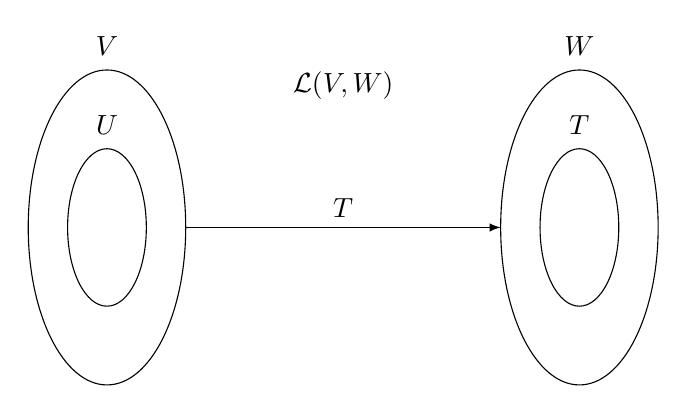
\begin{tikzpicture}[>=latex]
    % Define the main vector spaces
    \def\vsA{(0,0) ellipse (1cm and 2cm)}
    \def\vsB{(6,0) ellipse (1cm and 2cm)}

    % Draw the main vector spaces
    \draw \vsA node at (0,2.3) {$V$};
    \draw \vsB node at (6,2.3) {$W$};

    % Define the subspaces
    \def\subA{(0,0) ellipse (0.5cm and 1cm)}
    \def\subB{(6,0) ellipse (0.5cm and 1cm)}

    % Draw the subspaces
    \draw \subA node at (0,1.3) {$U$};
    \draw \subB node at (6,1.3) {$T$};

    % Define the linear transformation
    \draw[->] (1,0) -- node[above] {$T$} (5,0);

    % Define the label for the linear transformation
    \node at (3,1.8) {$\mathcal{L}(V,W)$};
  \end{tikzpicture}

  % \begin{tikzpicture}[>=latex]
  %   % Define the main vector spaces
  %   \def\vsA{(0,0) ellipse (1.5cm and 1cm)}
  %   \def\vsB{(6,0) ellipse (1.5cm and 1cm)}
  %   \def\vsC{(3,-3) ellipse (1.5cm and 1cm)}
  %
  %   % Draw the main vector spaces
  %   \draw \vsA node at (0,1) {$V$};
  %   \draw \vsB node at (6,1) {$W$};
  %   \draw \vsC node at (3,-4) {$U$};
  %
  %   % Define the subspaces
  %   \def\subA{(0,0) ellipse (0.8cm and 0.5cm)}
  %   \def\subB{(6,0) ellipse (0.8cm and 0.5cm)}
  %   \def\subC{(3,-3) ellipse (0.8cm and 0.5cm)}
  %
  %   % Draw the subspaces
  %   \draw \subA node at (0,0.8) {$U_1$};
  %   \draw \subB node at (6,0.8) {$W_1$};
  %   \draw \subC node at (3,-3.5) {$V_1$};
  %
  %   % Define the linear transformations
  %   \draw[->] (1.5,0) -- node[above] {$T$} (4.5,0);
  %   \draw[->] (0,-1) -- node[left] {$S$} (3,-2);
  %   \draw[->] (6,-1) -- node[right] {$R$} (3,-2);
  %
  %   % Define the labels for the linear transformations
  %   \node at (3,0.5) {$\mathcal{L}(V,W)$};
  %   \node at (1.5,-1.5) {$\mathcal{L}(U,V)$};
  %   \node at (4.5,-1.5) {$\mathcal{L}(U,W)$};
  % \end{tikzpicture}

  This marks the end of Chapter 3. Chapter 4 will focus on polynomial, and
  chapter 5 on determinants.

  We will study linear operators for some time, as they have a lot of real world
  significance.

  We will find a magic polynomial: the characteristic polynomial, which will
  give us a lot of information about the linear transformation.

  \subsection{Chapter 4}

  {\it Our discussion of polynomials begins}.

  {\bf Note}: We will mostly skip $4.1$ and $4.3$ from the book

  Let $F$ be a field ($\Q$, $\R$, $\C$). Which field we choose is going to
  matter here.

  \definition{
    $F[x]$ is all polynomials of the form

    \[
      a_0 + a_1 x + a_2 x^2 + \cdots + a_n x^n
    \]

    Where $a_0, a_1, \dots, a_n \in F$
  }

  We saw this before, we just called it $\P$ before. We also had that $\P$ had
  the basis $\{1, x, x^2, \dots\}$

  {\bf Note}: We can multiply two polynomials together and get a polynomial!

  You can always add, always subtract, always multiply, but not always divide!
  For instance you cant divide by the zero polynomial. There are restrictions
  about when you can divide.

  $f(x) = x^2$ is a perfectly fine polynomial, but $\frac{1}{x^2}$ is not a
  polynomial, since there is no multiplicative inverse. \TODO{} verify

  We say that $F[x]$ is a {\bf ring}.

  {\bf Note}: Every field is a ring, but not every ring is a field.

  As a side note, we can see that $\Q$ is a field, but $\Z$ is not: {\it it} is a ring.

  What we have in mind here, is to study linear operators $T: V \to V$.
  Polynomials are a tool for understanding these $T$s.

  Given, say $f(x) = x^2 + 2x - 3$, we can apply $f$ to $T$, getting $f(T)$

  \[
    f(T) = T^2 + 2T - 3(I)
  \]

  \btw{Remind yourself what $T^2$ means: it's $T \circ T$.}

  Which is itself a different linear transformation going from $V$ to $V$.

  Given such a $T$, we are interested in the set $J$ of all polynomials $f \in F[x]$
  such that $f(T)$ is the zero transformation.

  \[
    J = \Big\{ \text{polynomials } f \in F[x] \text{ such that } f(T) = \vec{0} \Big\}
  \]

  We'll see that, for any $T$, this is an {\bf ideal} of $F[x]$.

  Within such a $J$, there is a particular polynomial called the {\bf
  characteristic polynomial}.

  We'll see later that, how the characteristic polynomial factors will tell us a
  lot of information about $T$.

  But what do we mean by factoring?

  \definition{
    A polynomials $d(x)$ divides $f(x)$ if there is some other $q(x) \in F[x]$
    such that

    \[
      f = d \cdot q
    \]
  }

  We'll later try to factor this all the way down, similarly to the unique prime
  factorization of the natural numbers. We'll see that for a given polynomial
  $p$, we'll get a unique factorization.

  {\bf Danger}: For a particular $f(x)$, whether or not $f$ factors may depend
  on the field $F$. For example

  let $f(x) = x^2 + 1$. In $\R[x]$, $f$ is irreducible. But in $\C[x]$, $f$ does
  factor!

  \[
    x^2 + 1 = (x - i)(x + i)
  \]

  {\bf Notation}: The zero polynomial is always a special case. If we're trying
  to prove something for all polynomials, we tend to handle zero separately.

  For $f \in F[x], f \ne 0$, the {\bf degree} of $a_0 + a_1 x + \cdots + a_m
  x^m$ is the largest $n$ such that $a_i \ne 0$.

  We say that $f$ is {\bf monic} if $a_n = 1$, where $n$ is the degree of $2$.
  For example

  \[
    f(x) = x^2 + 2x - 3
  \]

  $f$ is a monic of degree 2, since the leading coefficient is 1.

  In the integers, we have the idea of the GCD, the largest number that divides
  all members of a set. For example

  \[
    \GCD(24, 36) = 12
  \]

  For polynomials, we can do something similar. Given $\{f_1, f_2, f_3\}$,
  $\GCD(f_1, f_2, f_3)$ is the polynomial $h$ of largest degree such that
  $h$ divides $f_1$, $f_2$, and $f_3$.


\end{document}
